%----------------------------------------------------------------------------------------
%    PACKAGES AND THEMES
%----------------------------------------------------------------------------------------

\documentclass[aspectratio=169,xcolor=dvipsnames]{beamer}
\usetheme{SimpleDarkBlue}

\usepackage{hyperref}
\usepackage{graphicx} % Allows including images
\usepackage{booktabs} % Allows the use of \toprule, \midrule and \bottomrule in tables
\usepackage{tikz}
\usetikzlibrary{shapes,arrows,positioning} 


\begin{document}



\title{ICP225 - Computação II}

\author{Prof. Gabriel Rodrigues Caldas de Aquino}

\institute
{
    gabrielaquino@ic.ufrj.br\\
    
    Instituto de Computação -
    Universidade Federal do Rio de Janeiro % Your institution for the title page
}
\date{Compilado em: \\ \today} % Date, can be changed to a custom date

%----------------------------------------------------------------------------------------
%    PRESENTATION SLIDES
%----------------------------------------------------------------------------------------

%------------------------------------------------
\section{Apresentação do curso}
%------------------------------------------------
\begin{frame}
    % Print the title page as the first slide
    \titlepage
\end{frame}



\begin{frame}{Método de Avaliação}
  \begin{block}{Componentes da Nota}
    \begin{itemize}
      \item \textbf{Provas (P1 e P2):}  
  Média das provas (MP) $\rightarrow$ 80\% da nota
      \item \textbf{Trabalhos:} 
  Média dos trabalhos (MT) $\rightarrow$ 20\% da nota 
    \end{itemize}
  \end{block}

  \begin{block}{Critério de Aprovação Direta}
    \begin{itemize}
      \item Média ponderada de MP e MT $\geq 7$ 
      \hspace{1em} $\rightarrow$ Aprovado direto
      \item Se $3 <= \text{Média ponderada de MP e MT } <= 7$ 
      \hspace{1em} $\rightarrow$ Prova final (PF)
    \end{itemize}
  \end{block}

  \begin{block}{Cálculo da Média Final}
    \[
      \text{Média final} = \frac{\text{Média anterior} + \text{PF}}{2}
    \]
    \begin{itemize}
      \item Se $\text{Média final} \geq 5$ $\Rightarrow$ Aprovado
      \item Caso contrário $\Rightarrow$ Reprovado
    \end{itemize}
  \end{block}
\end{frame}
\title{Revisão Inicial}

\author{Prof. Gabriel Rodrigues Caldas de Aquino}

\institute
{
    gabrielaquino@ic.ufrj.br\\
    
    Instituto de Computação -
    Universidade Federal do Rio de Janeiro % Your institution for the title page
}
\date{Compilado em: \\ \today} % Date, can be changed to a custom date

%----------------------------------------------------------------------------------------
%    PRESENTATION SLIDES
%----------------------------------------------------------------------------------------

%------------------------------------------------
\section{Revisão Inicial}
%------------------------------------------------

\begin{frame}
    % Print the title page as the first slide
    \titlepage
\end{frame}

\begin{frame}{Material de Referência}

\begin{block}{Site de Computação 1 - Python}
Acesse o conteúdo, exemplos e exercícios do curso de Computação 1 em:

\centering
\href{https://python.ic.ufrj.br/index.html}{\textbf{https://python.ic.ufrj.br/index.html}}

\vspace{1em}

Explore o material complementar, slides, desafios e mais recursos úteis para aprender Python.
\end{block}

\end{frame}



\begin{frame}[fragile]{Paradigmas de Programação}


\begin{block}{Paradigma de Programação}
\begin{itemize}
    \item \textbf{Padrão} para estruturação do programa.
    \item Organização da \textbf{solução algorítmica}.
    \item Exemplo em Python (imperativo estruturado):
    \begin{verbatim}
    def calcular_media(notas):
        soma = 0
        for n in notas:
            soma += n
        return soma / len(notas)
    \end{verbatim}
\end{itemize}
\end{block}
\end{frame}
\begin{frame}[fragile]{Estilos de Programação}
\begin{block}{Estilo de Programação}
\begin{itemize}
    \item \textbf{Organização do código} (legibilidade, manutenção).
    \item Influência no \textbf{raciocínio do programador}.
    \item Exemplo modular em Python:
    \begin{verbatim}
    def quadrado(x):
        return x ** 2

    print(quadrado(5))  # Saída: 25
    \end{verbatim}
\end{itemize}
\end{block}

\centering
\begin{itemize}
    \item Em Comp2: Evolução para POO (classes, herança) e outros paradigmas
 
\end{itemize}
\end{frame}



\begin{frame}[fragile]{Paradigma Imperativo}

\begin{block}{Paradigma Imperativo Estruturado}
\begin{itemize}
    \item Código sequencial
    \item "Faça isso, depois isso, depois aquilo…"
\end{itemize}
\begin{verbatim}
valor = int(input("Digite um número: "))
if valor > 0:
    print("Positivo")
    resultado = valor * 2
else:
    print("Negativo")
    resultado = valor + 10
print("Resultado:", resultado)
\end{verbatim}
\vspace{-0.3cm}

\end{block}
\end{frame}

\begin{frame}[fragile]{Estilo Modular}
\begin{block}{Estilo Modular}
\begin{itemize}
    \item Construção de módulos
    \item Pequenos códigos (módulos) que tem uma função única
    \item Evitar fazer códigos grandes
    \item A combinação dos módulos realiza uma grande tarefa
    \item Os módulos são as funções

\end{itemize}
\begin{verbatim}
# Módulo de processamento
def calcular(x):
    return x * 2 if x > 0 else x + 10
# Módulo de entrada e saída
def ler_imprimir():
    valor = int(input("Digite um número: "))
    print("Resultado:", calcular(valor))
ler_imprimir()
\end{verbatim}
\vspace{-0.3cm}

\end{block}


\end{frame}



\begin{frame}[fragile]{Tipos de Dados Básicos}
\begin{columns}[T]

\column{0.48\textwidth}
\begin{block}{Numéricos}
\begin{verbatim}
# Inteiro (int)
idade = 25

# Ponto flutuante (float)
peso = 68.5
\end{verbatim}
\end{block}

\column{0.48\textwidth}
\begin{block}{Texto (string)}
\begin{verbatim}
# String (str)
nome = "Maria"
msg = 'Olá, mundo!'
\end{verbatim}
\end{block}

\end{columns}

\begin{alertblock}{Características}
\begin{itemize}
    \item \texttt{int}: Valores inteiros (ex: -3, 0, 42)
    \item \texttt{float}: Decimais (ex: 3.14, -0.5)
    \item \texttt{str}: Texto (entre aspas simples ou duplas)
\end{itemize}
\end{alertblock}
\end{frame}

\begin{frame}[fragile]{Operações com Tipos Básicos}
\begin{columns}[T]

\column{0.48\textwidth}
\begin{block}{Numéricas}
\begin{verbatim}
soma = 5 + 3.2         #Result: 8.2
subtracao = 10 - 4     #Result: 6
multiplicacao = 7 * 2  #Result: 14
divisao = 15 / 2       #Result: 7.5
modulo = 10 % 3        #Result: 1
exponenciacao = 2 ** 3 #Result: 8
\end{verbatim}
\end{block}

\column{0.48\textwidth}
\begin{block}{Strings}
\begin{verbatim}
"a" + "b"   # "ab" (concatenação)
"oi" * 3    # "oioioi" (repetição)
len("abc")  # 3 (tamanho)
\end{verbatim}
\end{block}

\end{columns}

\begin{exampleblock}{Importante}
\begin{itemize}
    \item Não misture tipos! \texttt{"10" + 5} → Erro!
    \item Converta com \texttt{int()}, \texttt{str()}, etc.
\end{itemize}
\end{exampleblock}
\end{frame}

\begin{frame}[fragile]{Variáveis e Atribuição}

\begin{block}{O que são variáveis?}
\begin{itemize}
    \item \textbf{Armazenam informações} para uso futuro e são mantidas na \textbf{memória RAM}
    \item Acessadas através de um \textbf{identificador} (nome)
\end{itemize}
\end{block}

\begin{exampleblock}{Comando de Atribuição}
\begin{verbatim}
# Sintaxe: nome_variavel = valor
idade = 25             # Criando variável 'idade'
pi = 3.1415            # Atribuição de valor decimal
mensagem = "Olá!"      # Variável do tipo string
\end{verbatim}
\end{exampleblock}

\begin{alertblock}{Regras Importantes}
\begin{itemize}
    \item Nomes à \textbf{esquerda} do \texttt{=}, valores à \textbf{direita}
    \item Podem ser \textbf{reescritas}: \texttt{contador = 10} → \texttt{contador = 20}
    \item Tipos são \textbf{inferidos} automaticamente
\end{itemize}
\end{alertblock}
\end{frame}

\begin{frame}[fragile]{Funções em Python}


\begin{columns}
    \column{0.60\textwidth}
    \begin{block}{O que são funções?}
        \begin{itemize}
            \item \textbf{Trechos de código} com um objetivo específico
            \item \textbf{Organizam} e \textbf{dividem} problemas complexos
            \item Podem \textbf{retornar valores} ou executar ações
        \end{itemize}
    \end{block}
    
    \column{0.40\textwidth}
    \begin{alertblock}{Por que usar funções?}
        \begin{itemize}
            \item \textbf{Evita repetição} de código
            \item Facilita \textbf{manutenção}
            \item Permite \textbf{reuso} em diferentes partes do programa
        \end{itemize}
    \end{alertblock}
\end{columns}


\begin{exampleblock}{Sintaxe Básica}
\begin{verbatim}
def nome_funcao(argumentos):
    # Corpo da função
    return resultado
# Exemplo real:
def calcular_media(nota1, nota2):
    media = (nota1 + nota2) / 2
    return media
\end{verbatim}
\end{exampleblock}


\end{frame}

\begin{frame}[fragile]{Exemplo Prático de Funções com Reuso}



    \begin{block}{Código em Python}
\begin{verbatim}
def calcular_area(largura, altura):
    """Calcula área de um retângulo"""
    return largura * altura

# Reuso da função
parede = calcular_area(3, 2.5)
janela = calcular_area(1.2, 1.5)
porta = calcular_area(0.8, 2.1)

area_total = parede - janela - porta

print(f"Área para pintar: {area_total}m²")
\end{verbatim}
    \end{block}




\end{frame}

\begin{frame}[fragile]{Escopo de Variáveis em Funções - Cuidado!}
    \begin{exampleblock}{Exemplo Prático}
\begin{verbatim}
def calcular():
    x = 10  # Variável local
    print(x)

calcular()
print(x)  # ERRO! x não existe aqui
\end{verbatim}
    \end{exampleblock}
\begin{columns}[T]
    \column{0.5\textwidth}
    \begin{block}{\textbf{Escopo}: Conceito chave que  determina}
        
        \begin{itemize}
            \item \textbf{Tempo de vida}:\\ Quando a variável existe
            \item \textbf{Visibilidade}:\\ Onde a variável pode ser acessada
        \end{itemize}
    \end{block}


    \column{0.5\textwidth}
    \begin{alertblock}{Regras Importantes}
        \begin{itemize}
            \item Variáveis \textbf{dentro} da função:
            \begin{itemize}
                \item Nascem quando a função é chamada
                \item Morrem quando a função termina
                \item São \textbf{invisíveis} fora da função
            \end{itemize}
            \item \textbf{Cuidado}:\\ Tentar acessar fora causa erro
        \end{itemize}
    \end{alertblock}


\end{columns}


\end{frame}

\begin{frame}[fragile]{Strings em Python - Definição e Índices}

\begin{columns}[T]
    \column{0.5\textwidth}
    \begin{block}{Definição e Criação}
        \begin{itemize}
            \item Sequência imutável de caracteres
            \item Podem usar \texttt{' '} ou \texttt{" "}
            \item Exemplos:
\begin{verbatim}
disciplina = 'Computação 1'
nome = "Maria"
\end{verbatim}
        \end{itemize}
    \end{block}

    \begin{block}{Acesso por Índice}
        \begin{itemize}
            \item Posições começam em 0
            \item Índices negativos acessam do final
\begin{verbatim}
print(nome[0])   # 'M'
print(nome[-1])  # 'a'
\end{verbatim}
        \end{itemize}
    \end{block}

    \column{0.5\textwidth}
    \begin{exampleblock}{Tabela de Índices}
        \centering
        \begin{tabular}{|c|c|c|c|c|c|}
            \hline
            \textbf{Índice +} & 0 & 1 & 2 & 3 & 4 \\
            \hline
            \textbf{Caractere} & M & a & r & i & a \\
            \hline
            \textbf{Índice -} & -5 & -4 & -3 & -2 & -1 \\
            \hline
        \end{tabular}
    \end{exampleblock}

    \begin{block}{Imutabilidade de string}
        \begin{itemize}
            \item Strings são \textbf{imutáveis}
            \item Tentar modificar gera erro:
\begin{verbatim}
nome[0] = 'm'  # TypeError
\end{verbatim}
        \end{itemize}
    \end{block}
\end{columns}

\end{frame}


\begin{frame}[fragile]{Strings em Python - Operações Comuns}


    
    \begin{block}{Operações com Strings}
        \begin{itemize}
            \item \textbf{Concatenação (\texttt{+}):} Junta duas strings.
            \item \textbf{Repetição (\texttt{*}):} Repete a string várias vezes.
            \item \textbf{Tamanho (\texttt{len}):} Retorna o número de caracteres.
            \item \textbf{Pertencimento (\texttt{in}):} Verifica se uma substring está contida.
            \item \textbf{Fatiamento (\texttt{:}):} Retorna partes da string (substrings).
        \end{itemize}
    \end{block}


    \begin{block}{Exemplos}
\begin{verbatim}
len(nome)          # 5
nome + ' Silva'    # 'Maria Silva'
'ri' in nome       # True
'-' * 10           # '----------'
nome[1:4]          # 'ari'
\end{verbatim}
    \end{block}


\end{frame}


\begin{frame}[fragile]{Tudo sobre Strings em Python - Demonstração Prática}



\begin{verbatim}
nome = "Ana Clara"
idade = 22

print(nome[0], nome[-1])  # A a

print(nome[4:9])   # Clara
print(nome[:3])    # Ana

print(len(nome))           # 8
print("Ana" in nome)       # True
print(nome + " Silva")     # Ana Clara Silva

print(nome.split())        # ['Ana', 'Clara']

print(f"{nome} tem {idade} anos")  # Ana Clara tem 22 anos
\end{verbatim}
\end{frame}

\begin{frame}[fragile]{Tuplas em Python}

\begin{block}{Características das Tuplas}
\begin{itemize}
    \item Sequência de dados \textbf{ordenados}, representadas por \textbf{parênteses}.
    \item Podem conter \textbf{diferentes tipos} de dados: inteiros, floats, strings, outras tuplas etc.
    \item São \textbf{imutáveis}: não é possível alterar seus valores após a criação.
    \item São \textbf{indexadas}: acessamos os elementos por índices, como em listas ou strings.
    \item Suportam \textbf{fatiamento} (slicing).
\end{itemize}
\end{block}

\vspace{0.5em}

\begin{block}{Exemplo}
\begin{verbatim}
tuplanum = (1, 2, 3)
mistura = ('Maria', 10, 3.14, (1, 2))

print(tuplanum[0])    # 1
print(mistura[-1])    # (1, 2)
print(tuplanum[1:])   # (2, 3)
\end{verbatim}
\end{block}

\end{frame}


\begin{frame}[fragile]{Listas em Python}

\begin{columns}[T]
    \column{0.55\textwidth}
    \begin{block}{Características das Listas}
        \begin{itemize}
            \item Sequência de valores \textbf{ordenados}, representada por \textbf{colchetes}.
            \item Suporta \textbf{diferentes tipos} de dados: inteiros, floats, strings, outras listas etc.
            \item São \textbf{mutáveis}: é possível alterar, adicionar e remover elementos.
            \item São \textbf{indexadas}, como strings e tuplas.
        \end{itemize}
    \end{block}

    \begin{block}{Exemplo}
\begin{verbatim}
listanum = [1, 2, 3]
listanum[0] = 10
\end{verbatim}
    \end{block}

    \column{0.45\textwidth}
    \begin{exampleblock}{Tabela de Índices}
    \centering
    \begin{tabular}{|c|c|c|c|}
        \hline
        \textbf{Índice +} & 0 & 1 & 2 \\
        \hline
        \textbf{Elemento} & 1 & 2 & 3 \\
        \hline
        \textbf{Índice -} & -3 & -2 & -1 \\
        \hline
    \end{tabular}
    \end{exampleblock}
\end{columns}

\end{frame}

\begin{frame}[fragile]{Listas em Python - Operações Comuns}

\begin{columns}[T]
    \column{0.6\textwidth}
    \begin{block}{Operações com Listas}
        \begin{itemize}
            \item \textbf{Tamanho} (\texttt{len}): número de elementos da lista.
            \item \textbf{Adicionar} (\texttt{append}, \texttt{insert}): adiciona elementos.
            \item \textbf{Remover} (\texttt{remove}, \texttt{pop}): exclui elementos.
            \item \textbf{Concatenação} (\texttt{+}): junta duas listas.
            \item \textbf{Repetição} (\texttt{*}): repete os elementos da lista.
            \item \textbf{Pertencimento} (\texttt{in}): verifica se um valor está na lista.
            \item \textbf{Fatiamento} (\texttt{:}): retorna sublistas.
        \end{itemize}
    \end{block}

    \column{0.4\textwidth}
    \begin{block}{Exemplos}
\begin{verbatim}
lista = [1, 2, 3]
len(lista)     # 3
lista.append(4)# [1, 2, 3, 4]
lista.pop()    # [1, 2, 3]
[0] + lista    # [0, 1, 2, 3]
[1] * 3        # [1, 1, 1]
2 in lista     # True
lista[1:3]     # [2, 3]
\end{verbatim}
    \end{block}
\end{columns}

\end{frame}

\begin{frame}[fragile]{Dicionários em Python}

\begin{block}{Características dos Dicionários}
\begin{itemize}
    \item \textbf{Coleção não ordenada} de dados.
    \item Representada por \texttt{\{ \}} com pares \textbf{chave: valor}.
    \item Acesso aos valores é feito pelas \textbf{chaves}, e não por índices.
    \item Cada \textbf{chave é única} dentro do dicionário.
    \item Os dicionários são \textbf{mutáveis}: é possível alterar, adicionar e remover pares.
\end{itemize}
\end{block}

\vspace{0.5em}

\begin{block}{Exemplo}
\begin{verbatim}
produtos = {
    'farinha': 3.00,
    'feijão': 5.00,
    'leite': 4.25,
    'açúcar': 2.49 }
print(produtos['leite'])  # 4.25
\end{verbatim}
\end{block}

\end{frame}

\begin{frame}[fragile]{Dicionários em Python - Operações Comuns}


    \begin{block}{Principais Operações}
        \begin{itemize}
            \item \textbf{Adicionar ou atualizar elementos}: atribuindo um valor a uma nova chave.
            \item \textbf{Pertencimento} (\texttt{in}): verifica se uma \textbf{chave} está no dicionário.
            \item \textbf{Verificar existência de chave}: com \texttt{in} ou usando \texttt{get()}.
        \end{itemize}
    \end{block}


    \begin{block}{Exemplos}
\begin{verbatim}
produtos['arroz'] = 4.99
'feijão' in produtos       # True
'macarrão' in produtos     # False
preco = produtos.get('leite')
\end{verbatim}
    \end{block}


\end{frame}

\begin{frame}[fragile]{Booleanos em Python}

\begin{block}{O que são Booleanos?}
\begin{itemize}
    \item Tipo \texttt{bool} representa apenas dois valores: \texttt{True} e \texttt{False}.
    \item Usado para expressar condições lógicas.
    \item Muito comum em estruturas de decisão (como \texttt{if}).
\end{itemize}
\end{block}

\vspace{0.5em}

\begin{columns}[T]
    \column{0.5\textwidth}
    \begin{block}{Operadores de Comparação}
    \begin{itemize}
        \item \texttt{==} : Igual a
        \item \texttt{!=} : Diferente de
        \item \texttt{>}  : Maior que
        \item \texttt{>=} : Maior ou igual a
        \item \texttt{<}  : Menor que
        \item \texttt{<=} : Menor ou igual a
    \end{itemize}
    \end{block}

    \column{0.5\textwidth}
    \begin{block}{Exemplos}
\begin{verbatim}
5 > 3        # True
10 == 20     # False
7 != 4       # True
2 <= 2       # True
\end{verbatim}
    \end{block}
\end{columns}

\end{frame}

\begin{frame}[fragile]{Booleanos em Python - Operadores Lógicos}

\begin{block}{Conectando Expressões Booleanas}
\begin{itemize}
    \item \texttt{not} – \textbf{Não lógico}: inverte o valor lógico.
    \item \texttt{and} – \textbf{E lógico}: verdadeiro apenas se as duas expressões forem verdadeiras.
    \item \texttt{or} – \textbf{Ou lógico}: verdadeiro se pelo menos uma das expressões for verdadeira.
\end{itemize}
\end{block}

\vspace{0.5em}

\begin{columns}[T]
    \column{0.5\textwidth}
    \begin{block}{Exemplos}
\begin{verbatim}
not True       # False
not False      # True

True and True  # True
True and False # False
\end{verbatim}
    \end{block}

    \column{0.5\textwidth}
    \begin{block}{Mais Exemplos}
\begin{verbatim}
True or False   # True
False or False  # False

x = 5
x > 0 and x < 10     # True
not (x == 5)         # False
\end{verbatim}
    \end{block}
\end{columns}

\end{frame}

\begin{frame}[fragile]{Estrutura Condicional em Python}

\begin{block}{Decisões com \texttt{if} e \texttt{else}}
\begin{itemize}
    \item Em muitas situações, partes do código devem ser executadas apenas se certas condições forem verdadeiras.
    \item Para isso, usamos expressões booleanas com as estruturas \texttt{if} e \texttt{else}.
    \item O bloco \texttt{if} só será executado se a condição for \texttt{True}.
    \item Caso contrário, o bloco \texttt{else} (se presente) será executado.
\end{itemize}
\end{block}

\vspace{0.5em}

\begin{block}{Sintaxe}
\begin{verbatim}
if <condição>:
    <bloco if>
else:
    <bloco else>
\end{verbatim}
\end{block}

\end{frame}

\begin{frame}[fragile]{Exemplo de Estrutura Condicional}

\begin{block}{Problema}
Queremos verificar se uma pessoa pode votar.  
Se a idade for maior ou igual a 18 anos, ela pode votar.  
Caso contrário, ela não pode votar.
\end{block}

\vspace{1em}

\begin{block}{Código em Python}
\begin{verbatim}
idade = int(input("Digite sua idade: "))

if idade >= 18:
    print("Você pode votar.")
else:
    print("Você não pode votar.")
\end{verbatim}
\end{block}

\end{frame}

\begin{frame}[fragile]{Estrutura de Repetição em Python}

\begin{block}{O que são Loops?}
\begin{itemize}
    \item Permitem executar um trecho de código várias vezes durante a mesma execução.
    \item Úteis para automatizar tarefas repetitivas.
\end{itemize}
\end{block}

\vspace{0.5em}

\begin{block}{Tipos de Estruturas de Repetição}
\begin{itemize}
    \item \textbf{While:} repete enquanto uma condição booleana for verdadeira.
    \item \textbf{For:} itera sobre elementos de uma coleção (strings, listas, tuplas, etc.).
\end{itemize}
\end{block}

\vspace{0.5em}

\begin{block}{Exemplos}
\begin{verbatim}
while condicao:
    # bloco de código
for elemento in iteravel:
    # bloco de código
\end{verbatim}
\end{block}

\end{frame}


\begin{frame}[fragile]{Exemplo de Loop \texttt{while}}

\begin{block}{Contando de 1 a 5 com \texttt{while}}
\begin{verbatim}
contador = 1

while contador <= 5:
    print(contador)
    contador += 1
\end{verbatim}
\end{block}

\end{frame}


\begin{frame}[fragile]{Exemplo de Loop \texttt{for}}

\begin{block}{Iterando sobre uma lista com \texttt{for}}
\begin{verbatim}
nomes = ['Ana', 'Bruno', 'Carlos']

for nome in nomes:
    print(nome)
\end{verbatim}
\end{block}

\end{frame}

\begin{frame}[fragile]{Entrada de Dados em Python}

\begin{block}{Função \texttt{input()}}
\begin{itemize}
    \item Usada para ler dados digitados pelo usuário.
    \item Sempre retorna uma \textbf{string}.
    \item É necessário converter o valor se quisermos um número.
\end{itemize}
\end{block}

\vspace{1em}

\begin{block}{Exemplos}
\begin{verbatim}
nome = input("Digite seu nome: ")
idade = input("Digite sua idade: ")

# Convertendo para inteiro
idade = int(idade)

# Ou diretamente
idade = int(input("Digite sua idade: "))
\end{verbatim}
\end{block}

\end{frame}


\begin{frame}[fragile]{Saída de Dados em Python}

\begin{block}{Função \texttt{print()}}
\begin{itemize}
    \item Utilizada para \textbf{exibir informações} ao usuário.
    \item Pode mostrar textos, resultados de expressões, valores de variáveis, etc.
    \item Aceita múltiplos argumentos separados por vírgula.
\end{itemize}
\end{block}

\vspace{1em}

\begin{block}{Exemplos}
\begin{verbatim}
print("Olá, mundo!")
nome = "Maria"
print("Olá,", nome)

idade = 20
print("Idade:", idade)
\end{verbatim}
\end{block}

\end{frame}

\title{Programação Orientada a Objetos}

\author{Prof. Gabriel Rodrigues Caldas de Aquino}

\institute
{
    gabrielaquino@ic.ufrj.br\\

    Instituto de Computação -
    Universidade Federal do Rio de Janeiro % Your institution for the title page
}
\date{Compilado em: \\ \today} % Date, can be changed to a custom date

%----------------------------------------------------------------------------------------
%    PRESENTATION SLIDES
%----------------------------------------------------------------------------------------

%------------------------------------------------
\section{Revisão Inicial}
%------------------------------------------------

\begin{frame}
    % Print the title page as the first slide
    \titlepage
\end{frame}

\begin{frame}{Programação Orientada a Objetos}

    \begin{block}{O que é um Objeto?}
        \begin{itemize}
            \item Unidade de software que \textbf{encapsula dados e algoritmos}.
            \item Representa conceitos ou entidades do mundo real ou conceitual.
            \item Relaciona-se com outras entidades, assim como na vida cotidiana.
        \end{itemize}
    \end{block}

    \begin{block}{Por que usar?}
        \begin{itemize}
            \item Estruturação clara e organizada do código.
            \item Especialmente útil para \textbf{projetos extensos}.
            \item Facilita o desenvolvimento de sistemas:
                  \begin{itemize}
                      \item Modulares
                      \item Reutilizáveis
                      \item De fácil manutenção
                  \end{itemize}
        \end{itemize}
    \end{block}

\end{frame}

\begin{frame}[fragile]{Classe em Python}

    \begin{block}{O que é uma Classe?}
        \begin{itemize}
            \item Unidade inicial e mínima para código orientado a objetos.
            \item Abstrai conceitos, definições e comportamentos.
            \item Descreve atributos (dados) e métodos (ações) dos objetos.
            \item Objetos são \textbf{instanciados} a partir de classes.
        \end{itemize}
    \end{block}

    \begin{block}{Exemplo em Python}
        \begin{verbatim}
class Pessoa:
    def __init__(self, nome, idade):
        self.nome = nome
        self.idade = idade
    def apresentar(self):
        print(f"Olá, meu nome é {self.nome} e tenho {self.idade} anos.")
p1 = Pessoa("Maria", 20)
p1.apresentar()
\end{verbatim}
    \end{block}

\end{frame}

\begin{frame}[fragile]{Exemplo em Python - Personagem de RPG}

    \begin{verbatim}
class Personagem:
    def __init__(self, vida, forca, inteligencia):
        self.vida = vida
        self.forca = forca
        self.inteligencia = inteligencia
    def atacar(self):
        print("O personagem atacou!")
    def defender(self):
        print("O personagem defendeu!")
    def usar_magia(self):
        print("O personagem lançou uma magia!")
# Criando um objeto (instância) da classe
heroi = Personagem(100, 20, 15)
heroi.atacar()
print("Vida:", heroi.vida)
\end{verbatim}

\end{frame}


\begin{frame}[fragile]{Exemplo com Conceitos de POO}

    \begin{itemize}
        \item \textbf{Classe}:
              Projeto de um personagem de RPG.
        \item \textbf{Objeto}:
              Cada personagem criado com base nesse projeto.
    \end{itemize}

    \begin{itemize}
        \item \textbf{Atributos}
              \begin{itemize}
                  \item Vida
                  \item Força
                  \item Inteligência
              \end{itemize}
        \item \textbf{Métodos}
              \begin{itemize}
                  \item Atacar
                  \item Defender
                  \item Usar magia
              \end{itemize}

    \end{itemize}

    \begin{exampleblock}{Trecho de Código}
        \begin{verbatim}
heroi = Personagem(100, 20, 15)
heroi.atacar()
\end{verbatim}
    \end{exampleblock}

\end{frame}



\begin{frame}{Atributos em POO}

    \begin{block}{Definição}
        \begin{itemize}
            \item Representam as características do objeto.
            \item Definidos dentro da classe.
            \item Armazenam valores que caracterizam o objeto.
        \end{itemize}
    \end{block}

    \begin{exampleblock}{Exemplo: Classe \texttt{Personagem}}
        \begin{itemize}
            \item \textbf{vida} – Pontos de vida do personagem.
            \item \textbf{força} – Poder de ataque físico.
            \item \textbf{inteligência} – Capacidade para magia ou estratégias.
        \end{itemize}
    \end{exampleblock}

    \begin{block}{Observação}
        Cada objeto criado a partir da classe \texttt{Personagem} terá seus próprios valores para esses atributos.
    \end{block}

\end{frame}

\begin{frame}[fragile]{Métodos em POO}

    \begin{block}{Definição}
        \begin{itemize}
            \item São as ações que o objeto pode executar.
            \item Definidos como funções dentro da classe.
            \item Podem usar e alterar os atributos do objeto.
        \end{itemize}
    \end{block}

    \begin{exampleblock}{Exemplo: Classe \texttt{Personagem}}
        \begin{itemize}
            \item \textbf{atacar()} – Realiza um ataque.
            \item \textbf{defender()} – Executa defesa.
            \item \textbf{usar\_magia()} – Lança um feitiço.
        \end{itemize}
    \end{exampleblock}

    \begin{exampleblock}{Trecho de Código}
        \begin{verbatim}
heroi.defender()
heroi.usar_magia()
\end{verbatim}
    \end{exampleblock}

\end{frame}

\begin{frame}[fragile]{Método Construtor em Python}

    \begin{block}{Definição}
        \begin{itemize}
            \item Método especial chamado automaticamente ao criar um objeto.
            \item Usado para inicializar os atributos da nova instância.
            \item Em Python, o construtor é o método \texttt{\_\_init\_\_()}.
            \item O construtor:
                  \begin{itemize}
                      \item Facilita a inicialização de atributos obrigatórios.
                      \item Se não for definido, Python usa um construtor default que não faz nada.
                  \end{itemize}
        \end{itemize}
    \end{block}

    \begin{exampleblock}{Exemplo simples}
        \begin{verbatim}
class Personagem:
    def __init__(self, vida, forca):
        self.vida = vida
        self.forca = forca

heroi = Personagem(100, 20)
\end{verbatim}
    \end{exampleblock}

\end{frame}

\begin{frame}[fragile]{O parâmetro \texttt{self} em Métodos}

    \begin{block}{Definição}
        \begin{itemize}
            \item Deve ser o primeiro parâmetro em métodos de instância.
            \item Representa o próprio objeto que chama o método.
            \item Permite acessar atributos e outros métodos do objeto.
            \item É obrigatório explicitar no código, mas não na chamada do método.
        \end{itemize}
    \end{block}

    \begin{exampleblock}{Exemplo simples}
        \begin{verbatim}
class Personagem:
    def apresentar(self):
        print("Eu sou um personagem!")

p = Personagem()
p.apresentar()  # 'self' é passado automaticamente
\end{verbatim}
    \end{exampleblock}

\end{frame}
\begin{frame}[fragile]{Classe Personagem - Método \texttt{defender}}

    \begin{verbatim}
class Personagem:
    def __init__(self, vida, forca, inteligencia):
        self.vida = vida
        self.forca = forca
        self.inteligencia = inteligencia
    def defender(self, dano_recebido):
        dano_final = dano_recebido / 2
        self.vida -= dano_final
        print(f"{self} defendeu e recebeu {dano_final} de dano. Vida restante: {self.vida}")
    def __str__(self):
        return "Personagem"

heroi = Personagem(100, 20, 15)
heroi.defender(30)
print("Vida do heroi:", heroi.vida)
\end{verbatim}

\end{frame}

\begin{frame}[fragile]{Classe Personagem - Método \texttt{ganhar\_healthpack}}

    \begin{verbatim}
class Personagem:
    def __init__(self, vida, forca, inteligencia):
        self.vida = vida
        self.forca = forca
        self.inteligencia = inteligencia
    def defender(self, dano_recebido):
        dano_final = dano_recebido / 2
        self.vida -= dano_final
        print(f"{self} defendeu e recebeu {dano_final} de dano. Vida restante: {self.vida}")
    def ganhar_healthpack(self, vida_restaurada):
        self.vida += vida_restaurada
        print(f"{self} recebeu {vida_restaurada} de Healthpack. Vida restante: {self.vida}")
    def __str__(self):
        return "Personagem"
heroi = Personagem(100, 20, 15)
heroi.ganhar_healthpack(50)
\end{verbatim}

\end{frame}

\begin{frame}[fragile]{Deixando mais pessoal - Personagem com nome}

    \begin{verbatim}
class Personagem:
    def __init__(self, nome, vida, forca, inteligencia):
        self.nome = nome
        self.vida = vida
        self.forca = forca
        self.inteligencia = inteligencia

    def __str__(self):
        return self.nome

heroi = Personagem("Arthur", 100, 20, 15)
\end{verbatim}

\end{frame}

\begin{frame}[fragile]{Por que o \texttt{print} mostra o nome do personagem?}

    \begin{block}{O método \texttt{\_\_str\_\_()}}
        \begin{itemize}
            \item O Python usa o método especial \texttt{\_\_str\_\_()} para definir como representar um objeto como texto.
            \item Quando usamos \texttt{print(objeto)}, o Python chama \texttt{objeto.\_\_str\_\_()} automaticamente.
            \item No exemplo, \texttt{\_\_str\_\_()} foi definido para retornar o nome do personagem.
            \item Por isso, o \texttt{print(heroi)} exibe o nome ao invés do endereço de memória.
        \end{itemize}
    \end{block}

    \begin{exampleblock}{Trecho do código}
        \begin{verbatim}
def __str__(self):
    return self.nome
\end{verbatim}
    \end{exampleblock}

\end{frame}

\begin{frame}[fragile]{Método \texttt{atacar} com interação entre objetos}

    \begin{verbatim}
class Personagem:
    def __init__(self, nome, vida, forca, inteligencia):
        self.nome = nome
        self.vida = vida
        self.forca = forca
        self.inteligencia = inteligencia
    def atacar(self, alvo):
        dano = self.forca * 2
        alvo.vida -= dano
        print(f"{self} atacou {alvo} causando {dano} de dano!")
        print(f"Vida restante de {alvo}: {alvo.vida}")
    def __str__(self):
        return self.nome
heroi = Personagem("Arthur", 100, 20, 15)
inimigo = Personagem("Goblin", 80, 15, 10)
heroi.atacar(inimigo)
\end{verbatim}

\end{frame}

\begin{frame}{Discussão em Grupo: Modelando Tipos de Dano}

    \begin{block}{Desafio}
        Como podemos implementar diferentes tipos de dano em nosso jogo?

        \begin{itemize}
            \item Dano pode ser igual à força do personagem.
            \item Pode ser o dobro (exemplo: fogo contra planta).
            \item Pode ser metade (exemplo: água contra planta).
            \item Ou igual para ataques contra o mesmo tipo.
        \end{itemize}


        \begin{block}{Pontos para pensar}
            \begin{itemize}
                \item Como representar os tipos dos personagens e dos ataques?
                \item Como aplicar multiplicadores diferentes para cada tipo de dano?
                \item Qual estrutura de dados usar para armazenar essas regras?
                \item Como modificar o método \texttt{atacar} para considerar isso?
            \end{itemize}
        \end{block}

    \end{block}

\end{frame}


\begin{frame}[fragile]{Tipos de dano}


    \begin{verbatim}
class Personagem:
    def __init__(self, nome, vida, forca, inteligencia, tipo):
        (...)
        self.tipo = tipo  # 'fogo', 'planta', 'agua'
    def atacar(self, alvo):
        if self.tipo == "fogo" and alvo.tipo == "planta":
            dano = self.forca * 2
        elif self.tipo == "agua" and alvo.tipo == "planta":
            dano = self.forca * 0.5
        else:
            dano = self.forca
        alvo.vida -= dano
        print(f"{self} atacou {alvo} causando {dano} de dano!")
        print(f"Vida restante de {alvo}: {alvo.vida}")
heroi = Personagem("Arthur", 100, 20, 15, "fogo")
inimigo = Personagem("Treant", 80, 15, 10, "planta")
\end{verbatim}



\end{frame}
\begin{frame}{Exercício: Modelando Formas Geométricas}

    \textbf{Desafio:} Crie classes em Python para representar formas geométricas básicas.

    \begin{itemize}
        \item Comece com duas formas: \texttt{Retangulo} e \texttt{Circulo}.
        \item Cada classe deve ter:
              \begin{itemize}
                  \item Atributos para as dimensões (ex: base e altura para retângulo, raio para círculo).
                  \item Método para calcular a área.
                  \item Método para calcular o perímetro (ou circunferência no caso do círculo).
              \end{itemize}
        \item Crie objetos de cada classe e imprima a área e perímetro.
    \end{itemize}


\end{frame}

\begin{frame}[fragile]{Exemplo: Classe Retângulo}

    \begin{block}{Classe \texttt{Retangulo}}
        \begin{verbatim}
class Retangulo:
def init(self, base, altura):
self.base = base
self.altura = altura
def area(self):
    return self.base * self.altura
def perimetro(self):
    return 2 * (self.base + self.altura)
\end{verbatim}
    \end{block}
\end{frame}
\begin{frame}[fragile]{Exemplo: Classe Círculo}

    \begin{block}{Classe \texttt{Circulo}}
        \begin{verbatim}
class Circulo:
def init(self, raio):
self.raio = raio
def area(self):
    return 3.1416 * self.raio ** 2

def perimetro(self):
    return 2 * 3.1416 * self.raio
\end{verbatim}
    \end{block}

\end{frame}

\title{POO - Herança e Polimorfismo}

\author{Prof. Gabriel Rodrigues Caldas de Aquino}

\institute
{
    gabrielaquino@ic.ufrj.br\\

    Instituto de Computação -
    Universidade Federal do Rio de Janeiro % Your institution for the title page
}
\date{Compilado em: \\ \today} % Date, can be changed to a custom date

%----------------------------------------------------------------------------------------
%    PRESENTATION SLIDES
%----------------------------------------------------------------------------------------

%------------------------------------------------
\section{Revisão Inicial}
%------------------------------------------------

\begin{frame}
    % Print the title page as the first slide
    \titlepage
\end{frame}


\begin{frame}{Encapsulamento}

    \begin{itemize}
        \item \textbf{Objetivo}: Esconder os detalhes internos de uma classe e expor apenas o que for necessário por meio de uma interface controlada

        \item \textbf{Ideia}: Os atributos (dados) de um objeto fiquem protegidos contra acessos e modificações indevidas, e que a interação externa aconteça de forma controlada através de métodos
    \end{itemize}



    \begin{block}{Então, basicamente:}
        \begin{itemize}
            \item Você coloca os dados e os métodos que operam sobre esses dados dentro da mesma classe.

            \item Controla quem pode acessar ou modificar esses dados usando modificadores de acesso (como público, protegido, privado).

            \item Com isso, aumenta a segurança, reutilização e manutenibilidade do código.
        \end{itemize}
    \end{block}

\end{frame}





\begin{frame}{Encapsulamento}

    \begin{block}{Então, na aula passada criamos métodos e os atributos...}
        \begin{itemize}
            \item Precisamos agora definir a visibilidade para atributos e métodos.
            \item Ver como podemos controlar o acesso e a manipulação dos dados da classe.

            \item Com isso vamos expor apenas o necessário para o uso correto da classe.

            \item O Fim é proteger a integridade dos dados, escondendo detalhes internos.
                  \begin{itemize}
                      \item Usuários sabem o que a classe faz, mas não como ela faz.
                      \item Permite alterar a implementação sem impactar código externo.
                  \end{itemize}
        \end{itemize}
    \end{block}



    \begin{block}{Níveis de acesso (\textcolor{yellow}{\textbf{Convenção do Python!}})}
        \begin{itemize}
            \item \textbf{Público}: acessível de qualquer lugar.
            \item \textbf{Protegido} (\_): acessível na classe e subclasses.
            \item \textbf{Privado} (\_\_): acessível apenas dentro da própria classe.

        \end{itemize}
    \end{block}

\end{frame}

\begin{frame}[fragile]{Métodos Protegidos e Privados em Python}
    \begin{itemize}
        \item \textbf{Métodos Protegidos (\texttt{\_método})}
              \begin{itemize}
                  \item Prefixados com \texttt{\_}.
                  \item Indicativo para programadores: não usar fora da classe.
                  \item \textbf{Não impedem} o acesso externo — podem ser chamados normalmente.
                  \item São uma \textbf{convenção} para organizar o código.
              \end{itemize}
        \item \textbf{Métodos Privados (\texttt{\_\_método})}
              \begin{itemize}
                  \item Prefixados com \texttt{\_\_}.
                  \item Python faz \textbf{name mangling} para dificultar o acesso externo.
                  \item Ainda podem ser acessados, mas não diretamente — é desencorajado.
                  \item Oferecem um nível maior de “proteção” que métodos protegidos.
              \end{itemize}
    \end{itemize}







\end{frame}


\begin{frame}[fragile]{Atributos e Métodos Públicos}

    \begin{itemize}
        \item \textbf{Atributos Públicos}
              Podem ser acessados e modificados diretamente fora da classe.
        \item \textbf{Métodos Públicos}
              Também podem ser chamados livremente de fora da classe.
    \end{itemize}




    \begin{exampleblock}{Exemplo em Python}
        \begin{verbatim}
class Pessoa:
    def __init__(self, nome, idade):
        self.nome = nome      # atributo público
        self.idade = idade    # atributo público
    def apresentar(self):     # método público
        print(f"Meu nome é {self.nome} e tenho {self.idade} anos.")
p = Pessoa("João", 30)
print(p.nome)       # acesso direto ao atributo público
p.idade = 31       # modificação direta
p.apresentar()      # chamada do método público
\end{verbatim}
    \end{exampleblock}

\end{frame}

\begin{frame}[fragile]{Métodos Protegidos}

    \begin{block}{Definição}
        Métodos protegidos não devem ser acessados ou modificados diretamente fora da classe. \textbf{Servem para detalhes internos}. Na \textbf{prática, é possível}, mas não foi feito para ser chamado diretamente por código externo.
    \end{block}

    \begin{exampleblock}{Exemplo em Python}
        \begin{verbatim}
class Pessoa:
    def __init__(self, nome):
        self.nome = nome

    def _falar(self):   # método protegido (convenção)
        print(f"{self.nome} está falando...")

p = Pessoa("Ana")
p._falar()   # possível, mas não recomendado acessar diretamente
\end{verbatim}
    \end{exampleblock}

\end{frame}


\begin{frame}[fragile]{Exemplo de Método Protegido}

    \begin{verbatim}
class Documento:
    def __init__(self, conteudo):
        self.conteudo = conteudo
        
    def _validar_tamanho(self):   # protegido
        return len(self.conteudo) > 0
        
    def salvar(self):             # público
        if self._validar_tamanho():
            print("Documento salvo.")
        else:
            print("Erro: documento vazio.")

    def exportar_pdf(self):        # público
        if self._validar_tamanho():  
            print("Relatório exportado em PDF.")
\end{verbatim}

\end{frame}


\begin{frame}[fragile]{Métodos Privados}

    \begin{block}{Definição}
        Métodos privados são usados para \textbf{detalhes internos da classe} que não devem ser acessados ou modificados fora dela.
        No Python, começam com \texttt{\_\_} (dois underlines) e sofrem \textbf{name mangling}, dificultando o acesso externo.
    \end{block}

    \small
    \begin{verbatim}
class Conta:
    def __init__(self, saldo):
        self.__saldo = saldo
    def __log_operacao(self, msg):   # método privado
        print(f"[LOG] {msg}")
    def depositar(self, valor):      # método público
        self.__saldo += valor
        self.__log_operacao(f"Depósito de {valor}")
c = Conta(100)
c.depositar(50)
# c.__log_operacao("teste")  # Erro: acesso direto proibido
\end{verbatim}


\end{frame}


\begin{frame}[fragile]{Exemplo de Método Privado em Python}
    \small
    \begin{verbatim}
class ContaBancaria:
    def __init__(self, saldo):
        self.__saldo = saldo  # atributo privado
    def depositar(self, valor):
        if valor > 0:
            self.__adicionar_saldo(valor)
            print(f"Depositado: {valor}")
    def __adicionar_saldo(self, valor):
        self.__saldo += valor
    def mostrar_saldo(self):
        print(f"Saldo atual: {self.__saldo}")
conta = ContaBancaria(100)
conta.depositar(50)
conta.mostrar_saldo()
# conta.__adicionar_saldo(100)  # Isso gera erro!
conta._ContaBancaria__adicionar_saldo(100)
conta.mostrar_saldo()
\end{verbatim}

\end{frame}




\begin{frame}[fragile]{Name Mangling em Python}

    \begin{block}{O que é Name Mangling?}
        \begin{itemize}
            \item Técnica do Python para “esconder” atributos/métodos privados.
            \item Atributos que começam com \_\_ (dois underlines) são renomeados internamente.
            \item Exemplo: \texttt{\_\_saldo} vira \texttt{\_NomeDaClasse\_\_saldo}.
            \item Evita acesso direto acidental e conflitos em herança.
        \end{itemize}
    \end{block}

    \begin{block}{Importante}
        \begin{itemize}
            \item Não é proteção total, apenas dificulta o acesso direto.
            \item Ainda é possível acessar via \texttt{\_NomeDaClasse\_\_atributo}, mas não recomendado.
            \item Indica que o membro é “privado” e não deve ser acessado externamente.
        \end{itemize}
    \end{block}
\end{frame}


\begin{frame}[fragile]{Name Mangling em Python}
    \begin{exampleblock}{Exemplo}
        \begin{verbatim}
class Conta:
def init(self):
self.__saldo = 100

c = Conta()
print(c._Conta__saldo) # Acesso via name mangling 
#(funciona, mas não é recomendado)
\end{verbatim}
    \end{exampleblock}

\end{frame}

\begin{frame}{Herança}

    \begin{block}{Definição}
        \begin{itemize}
            \item Herança é o relacionamento entre classes em que uma classe chamada de
                  \textbf{subclasse} (ou classe filha) é uma \textbf{extensão} ou \textbf{subtipo}
                  de outra classe chamada de \textbf{superclasse} (ou classe pai/mãe).

            \item A subclasse consegue \textbf{reaproveitar os atributos e métodos} da superclasse.
                  Além do que for herdado, a subclasse pode definir seus próprios membros
                  (atributos e métodos).
        \end{itemize}


    \end{block}

\end{frame}

\begin{frame}[fragile]{Herança e o uso do \texttt{super()}}

    \begin{block}{Relação de Herança}
        Estabelecemos a relação de herança ao indicar a \textbf{superclasse} entre parênteses na definição da subclasse:

        \begin{verbatim}
class Subclasse(Superclasse):
    ...
\end{verbatim}
    \end{block}

    \begin{block}{Uso do \texttt{super()}}
        Utilizamos o método \texttt{super()} para acessar a superclasse e, então, \textbf{reaproveitar seu construtor ou outros métodos}:

        \begin{verbatim}
class Aluno(Pessoa):
    def __init__(self, nome, cpf, dre):
        super().__init__(nome, cpf)  # chama __init__ de Pessoa
        self.dre = dre
\end{verbatim}
    \end{block}

\end{frame}

\begin{frame}[fragile]{O que é \texttt{super()}}
    \begin{itemize}
        \item \texttt{super()} retorna um objeto temporário da superclasse.
        \item Permite chamar métodos da superclasse sem repetir código.
        \item Fundamental para reaproveitar atributos e lógica já definida.
    \end{itemize}

\end{frame}



\begin{frame}[fragile]{Exemplo de Herança: Classe Aluno}

    \small

    \begin{verbatim}
class Pessoa:
    def __init__(self, nome):
        self.nome = nome
    def print_nome(self):
        print(self.nome)
class Aluno(Pessoa):   # Aluno herda de Pessoa
    def __init__(self, nome, matricula):
        super().__init__(nome)    # chama o construtor da superclasse
        self.matricula = matricula
    def inscrever_disciplina(self, disciplina):
        print(f"{self.nome} inscrito em {disciplina}")
    def exibir_informacoes(self):
        print(f"Nome: {self.nome}")
        print(f"Matrícula: {self.matricula}")
a = Aluno("Maria", "2025001")
a.inscrever_disciplina("Comp 2")
a.exibir_informacoes()
\end{verbatim}

\end{frame}



\begin{frame}[fragile]{Exemplo 2: Pessoa, aluno e professor}

    \small
    \begin{verbatim}
class Pessoa:
    def __init__(self, nome, cpf):
        self.nome = nome
        self.cpf = cpf
    def print_dados_pessoais(self):
        print(f"Nome: {self.nome}, CPF: {self.cpf}")
class Aluno(Pessoa):
    def __init__(self, nome, cpf, dre):
        super().__init__(nome, cpf)
        self.dre = dre
    def print_dados_aluno(self):
        print(f"Nome: {self.nome}, CPF: {self.cpf}, DRE: {self.dre}")
class Professor(Pessoa):
    def __init__(self, nome, cpf, siape):
        super().__init__(nome, cpf)
        self.siape = siape
    def print_dados_professor(self):
        print(f"Nome: {self.nome}, CPF: {self.cpf}, Siape: {self.siape}")

a = Aluno("Maria", "123.456.789-00", "2025001")
pr = Professor("João", "987.654.321-00", "112233")
pe = Pessoa("Pedro", "111.222.333-44")

a.print_dados_aluno()
pr.print_dados_professor()
pe.print_dados_pessoais()
\end{verbatim}

\end{frame}


\begin{frame}[fragile]{Função \texttt{isinstance()}}

    \begin{block}{Definição}
        A função \texttt{isinstance(objeto, classe)} verifica se um objeto é uma instância de uma classe específica ou de suas subclasses.

        \begin{itemize}
            \item Retorna \texttt{True} se o objeto for da classe ou de uma subclasse.
            \item Retorna \texttt{False} caso contrário.
        \end{itemize}
    \end{block}

    \begin{exampleblock}{Exemplo em Python}
        \begin{verbatim}
class Pessoa:
    pass
class Aluno(Pessoa):
    pass
a = Aluno()
print(isinstance(a, Aluno))   # True
print(isinstance(a, Pessoa))  # True, pois Aluno herda Pessoa
print(isinstance(a, dict))    # False
\end{verbatim}
    \end{exampleblock}

\end{frame}

\begin{frame}{Polimorfismo em POO}

    \begin{block}{Definição}
        Polimorfismo significa que o \textbf{significado de uma operação depende do objeto} em que ela é aplicada.
        Ou seja, o código não precisa se importar com o tipo exato do objeto, apenas com o que ele faz.
    \end{block}

    \begin{block}{Polimorfismo e Sobrescrita}
        Na prática, o polimorfismo ocorre principalmente através da \textbf{sobrescrita de métodos}:

        \begin{itemize}
            \item Subclasses podem redefinir métodos da superclasse.
            \item Estabelece uma \textbf{interface comum} para todas as classes que herdam da mesma superclasse.
        \end{itemize}
    \end{block}

    \begin{block}{Benefício}
        Podemos manipular objetos da superclasse de forma genérica, sem nos preocupar com a subclasse exata, sabendo que todos implementam os métodos comuns.
        O comportamento dos métodos pode variar dependendo da subclasse do objeto.
    \end{block}

\end{frame}


\begin{frame}[fragile]{Exemplo de Polimorfismo: Animais}

    \begin{exampleblock}{Definição de classes e métodos}
        \begin{verbatim}
class Animal:
    def fazer_som(self):
        print("arrrww")   # som genérico

class Gato(Animal):
    def fazer_som(self):
        print("miau")     # sobrescreve o som

class Cachorro(Animal):
    def fazer_som(self):
        print("auau")    # sobrescreve o som

# Lista de animais
animais = [Animal(), Gato(), Cachorro()]

for a in animais:
    a.fazer_som()   # polimorfismo: cada objeto responde de forma diferente
\end{verbatim}
    \end{exampleblock}

    \begin{block}{Saída Esperada}
        \begin{verbatim}
arrrww
miau
auau
\end{verbatim}
    \end{block}

\end{frame}


\begin{frame}[fragile]{Exemplo de Polimorfismo: Aprovação em Disciplina}


    \begin{verbatim}
class Aluno:
    def __init__(self, nome):
        self.nome = nome
    def verifica_aprovacao(self):
        pass  # método genérico, será sobrescrito
class Graduacao(Aluno):
    def verifica_aprovacao(self, nota, frequencia):
        return nota >= 5 and frequencia >= 75
class PosGraduacao(Aluno):
    def verifica_aprovacao(self, conceito, frequencia):
        return conceito in ["A", "B", "C"] and frequencia >= 75
a1 = Graduacao("Maria")
a2 = PosGraduacao("João")
print(a1.verifica_aprovacao(6, 80))    
print(a2.verifica_aprovacao("B", 90))  
\end{verbatim}




\end{frame}


\title{POO - Métodos Mágicos}

\author{Prof. Gabriel Rodrigues Caldas de Aquino}

\institute
{
    gabrielaquino@ic.ufrj.br\\
    
    Instituto de Computação -
    Universidade Federal do Rio de Janeiro % Your institution for the title page
}
\date{Compilado em: \\ \today} % Date, can be changed to a custom date

%----------------------------------------------------------------------------------------
%    PRESENTATION SLIDES
%----------------------------------------------------------------------------------------

%------------------------------------------------
\section{Revisão Inicial}
%------------------------------------------------

\begin{frame}
    % Print the title page as the first slide
    \titlepage
\end{frame}

\begin{frame}{Métodos Mágicos (Dunder)}

\begin{block}{Definição}
Métodos Mágicos são métodos pré-definidos que podem ser sobrescritos para definir como os objetos de uma classe irão interagir com operadores, funções específicas e instruções da linguagem Python.
\end{block}

\begin{block}{Características}
\begin{itemize}
    \item O nome dos métodos mágicos \textbf{inicia e termina com dois underlines} (\_\_).
    \item Também são chamados de \textbf{métodos Dunder} (“Double Underscore”).
    \item Permitem personalizar comportamento de operadores e funções nativas, como:
    \begin{itemize}
        \item \_\_str\_\_ → define como o objeto é convertido em string
        \item \_\_add\_\_ → define o comportamento do operador +
    \end{itemize}
\end{itemize}
\end{block}

\end{frame}

\begin{frame}[fragile]{Método Mágico \_\_str\_\_}

\begin{block}{Relembrando}
O método \texttt{\_\_str\_\_} é um dos métodos mágicos que já vimos e é usado para definir como um objeto será convertido em string.  
Ele é chamado automaticamente quando usamos o \texttt{print} com um objeto.
\end{block}

\begin{exampleblock}{Exemplo}
\begin{verbatim}
class Pessoa:
    def __init__(self, nome, idade):
        self.nome = nome
        self.idade = idade
    def __str__(self):
        return f"{self.nome}, {self.idade} anos"
p = Pessoa("Maria", 20)
print(p)   # chama automaticamente p.__str__()
# Saída: Maria, 20 anos
\end{verbatim}
\end{exampleblock}

\end{frame}


\begin{frame}{Alguns Métodos Mágicos (Dunder)}

\begin{columns}[T] % T para alinhamento no topo

\begin{column}{0.48\textwidth}
\begin{block}{Operadores Aritméticos}
\begin{tabular}{ll}
\texttt{\_\_add\_\_(self, other)} & + \\
\texttt{\_\_sub\_\_(self, other)} & - \\
\texttt{\_\_mul\_\_(self, other)} & * \\
\texttt{\_\_truediv\_\_(self, other)} & / \\
\texttt{\_\_floordiv\_\_(self, other)} & // \\
\texttt{\_\_mod\_\_(self, other)} & \% \\
\texttt{\_\_pow\_\_(self, other)} & **
\end{tabular}
\end{block}
\end{column}

\begin{column}{0.48\textwidth}
\begin{block}{Operadores de Comparação e Condicionais}
\begin{tabular}{ll}
\texttt{\_\_eq\_\_(self, other)} & == \\
\texttt{\_\_ne\_\_(self, other)} & != \\
\texttt{\_\_lt\_\_(self, other)} & $<$ \\
\texttt{\_\_le\_\_(self, other)} & $<=$ \\
\texttt{\_\_gt\_\_(self, other)} & $>$ \\
\texttt{\_\_ge\_\_(self, other)} & $>=$ \\
\texttt{\_\_contains\_\_(self, other)} & in
\end{tabular}
\end{block}
\end{column}

\end{columns}

\end{frame}



\begin{frame}[fragile]{Sobrescrita do operador + (\_\_add\_\_)}

\begin{verbatim}
class ContaBancaria:
    def __init__(self, banco, saldo):
        self.banco = banco
        self.saldo = saldo
    def __add__(self, outra):
        return self.saldo + outra.saldo
    def __str__(self):
        return f"{self.banco}: R$ {self.saldo}"
c1 = ContaBancaria("Santander", 1000)
c2 = ContaBancaria("Itau", 500)
print(c1 + c2)   # 1500
\end{verbatim}


\end{frame}
\begin{frame}[fragile]{Sobrescrita do operador  $>$ (\_\_gt\_\_)}


\begin{verbatim}
class ContaBancaria:
    def __init__(self, banco, saldo):
        self.banco = banco
        self.saldo = saldo
    def __gt__(self, outra):
        return self.saldo > outra.saldo
    def __str__(self):
        return f"{self.banco}: R$ {self.saldo}"
c1 = ContaBancaria("Bradesco", 1000)
c2 = ContaBancaria("Banco do Brasil", 500)
if c1 > c2:
    print(f"A conta {c1.banco} tem mais dinheiro")
else:
    print(f"A conta {c2.banco} tem mais dinheiro")

\end{verbatim}

\end{frame}

\begin{frame}{Alguns Outros Métodos Mágicos (Dunder)}

\begin{block}{Funções Comuns}
\begin{tabular}{ll}
\texttt{\_\_repr\_\_(self)} & \texttt{repr()} \\
\texttt{\_\_str\_\_(self)} & \texttt{str()} \\
\texttt{\_\_len\_\_(self)} & \texttt{len()} \\
\texttt{\_\_abs\_\_(self)} & \texttt{abs()} \\
\end{tabular}
\end{block}

\begin{block}{Operadores em Objetos Indexáveis}
\begin{tabular}{ll}
\texttt{\_\_getitem\_\_(self, key)} & \texttt{x = obj[key]} \\
\texttt{\_\_setitem\_\_(self, key, value)} & \texttt{obj[key] = value} \\
\texttt{\_\_delitem\_\_(self, key)} & \texttt{del obj[key]} \\
\end{tabular}
\end{block}

\begin{block}{Instruções Especiais}
\begin{tabular}{ll}
\texttt{\_\_iter\_\_(self), \_\_next\_\_(self)} & \texttt{for} \\
\texttt{\_\_enter\_\_(self), \_\_exit\_\_(self, exc\_type, exc\_value, traceback)} & \texttt{with} \\
\end{tabular}
\end{block}

\end{frame}

\begin{frame}[fragile]{Exemplo de \_\_getitem\_\_}

\begin{exampleblock}{Classe que armazena notas de uma disciplina}
\begin{verbatim}
class  Notas_disciplina:
    def __init__(self, disciplina, notas):
        self.disciplina = disciplina
        self.notas = notas  # lista de notas

    def __getitem__(self, indice):
        # permite acessar notas como se fosse uma lista
        return self.notas[indice]

Comp2 = Notas_disciplina("Comp2", [7, 8, 9, 10])

print(Comp2[0])  # 7
print(Comp2[2])  # 9
\end{verbatim}
\end{exampleblock}




\end{frame}


\title{POO - Classe Abstrata}

\author{Prof. Gabriel Rodrigues Caldas de Aquino}

\institute
{
    gabrielaquino@ic.ufrj.br\\
    
    Instituto de Computação -
    Universidade Federal do Rio de Janeiro % Your institution for the title page
}
\date{Compilado em: \\ \today} % Date, can be changed to a custom date

%----------------------------------------------------------------------------------------
%    PRESENTATION SLIDES
%----------------------------------------------------------------------------------------

%------------------------------------------------
\section{Revisão Inicial}
%------------------------------------------------

\begin{frame}
    % Print the title page as the first slide
    \titlepage
\end{frame}
%------------------------------------------------




\begin{frame}{Classes Abstratas na POO}
    Um componente do desenvolvimento moderno de software é a 
    \textbf{Programação Orientada a Objetos (POO)}, 
    que permite organizar o código de forma 
    \textbf{escalável}, \textbf{modular} e \textbf{reutilizável}. 
    
    \vspace{0.3cm}
    As \textbf{classes abstratas} são um dos conceitos centrais da POO, 
    fundamentais para criar um \textbf{modelo} (template) que outras classes podem usar.

\begin{block}{Pergunta}
    O que vocês acham que é uma classe abstrata?
\end{block}
\end{frame}


\begin{frame}{Classe Abstrata em POO}

\begin{block}{Definição}
\begin{itemize}
    \item Uma \textbf{classe abstrata} é uma classe que não pode ser instanciada diretamente.
    \item Atua apenas como base (superclasse) para outras classes.
    \item Pode conter:
    \begin{itemize}
        \item \textbf{Métodos implementados}: já possuem código definido.
        \item \textbf{Métodos abstratos}: devem obrigatoriamente ser sobrescritos nas subclasses concretas.
    \end{itemize}
\end{itemize}
\end{block}

\begin{block}{Objetivo}
Garantir que certas operações sejam obrigatoriamente implementadas pelas subclasses, definindo uma interface comum.
\end{block}

\end{frame}

\begin{frame}{O que é uma Classe Abstrata?}
    Uma \textbf{classe abstrata} é como um \textbf{molde} (ou \textbf{template}) para outras classes.  
    Ela define métodos que devem estar presentes em qualquer classe que herde dela, 
    mas não fornece o código específico desses métodos.
    
    \vspace{0.3cm}
    Pense nela como um \textbf{esqueleto mas sem dizer como preencher o resto}.
\end{frame}


\begin{frame}{Por que usar Classes Abstratas?}
    \begin{itemize}
        \item Definem um \textbf{molde} para outras classes.
        \item Obrigam a implementação de métodos específicos nas subclasses.
        \item Melhoram a \textbf{organização} e a \textbf{reutilização} do código.
        \item Permitem \textbf{polimorfismo}, ou seja, diferentes objetos 
              compartilhando uma interface comum.
    \end{itemize}
\end{frame}


\begin{frame}{Exemplo de Classe Abstrata}
    Suponha que você está construindo um programa para calcular a área de diferentes formas geométricas.

    \begin{itemize}
        \item Você cria uma \textbf{classe abstrata} chamada \texttt{Forma}, que define que toda forma deve ter um método \texttt{area()}.
        \item Mas \texttt{Forma} não especifica como \texttt{area()} funciona, pois a fórmula depende do tipo de forma.
        \item Cada forma específica (como \texttt{Circulo} ou \texttt{Retangulo}) herda de \texttt{Forma} e fornece sua própria implementação de \texttt{area()}.
    \end{itemize}
\end{frame}

\begin{frame}[fragile]{Antes das Classes Abstratas}

\small
\begin{verbatim}
class Forma:
    pass
    def area(self):
      pass
class Retangulo(Forma):
    def __init__(self, largura, altura):
        self.largura = largura
        self.altura = altura
    def area(self):
        return self.largura * self.altura
class Circulo(Forma):
    def __init__(self, raio):
        self.raio = raio
    def area(self):
        import math
        return 3.14 * self.raio**2
\end{verbatim}

\end{frame}

\begin{frame}[fragile]{Depois das classes abstratas}

\small
\begin{verbatim}
from abc import ABC, abstractmethod
# Classe abstrata
class Forma(ABC):
    @abstractmethod
    def area(self):
        pass
    @abstractmethod
    def perimetro(self):
        pass
# Subclasse concreta
class Circulo(Forma):
    def __init__(self, raio):
        self.raio = raio
    def area(self):
        return 3.14159 * self.raio ** 2
    def perimetro(self):
        return 2 * 3.14159 * self.raio
\end{verbatim}

\end{frame}

\begin{frame}[fragile]{Exemplo Completo de Classe Abstrata}
\small
\begin{columns}[T]

\begin{column}{0.48\textwidth}
\begin{verbatim}
from abc import ABC, abstractmethod
class Forma(ABC):
    @abstractmethod
    def area(self):
        pass
    @abstractmethod
    def perimetro(self):
        pass
class Circulo(Forma):
    def __init__(self, raio):
        self.raio = raio
    def area(self):
        return 3.14159 * self.raio ** 2
    def perimetro(self):
        return 2 * 3.14159 * self.raio
\end{verbatim}
\end{column}

\begin{column}{0.48\textwidth}
\begin{verbatim}
class Retangulo(Forma):
    def __init__(self, largura,
    altura):
        self.largura = largura
        self.altura = altura

    def area(self):
        return self.largura
        * self.altura

    def perimetro(self):
        return 2 * (self.largura
        + self.altura)
\end{verbatim}
\end{column}

\end{columns}
\end{frame}



\begin{frame}{Por que usar Classes Abstratas em Python?}

As classes abstratas são úteis quando queremos:

\begin{itemize}
    \item \textbf{Garantir a implementação de métodos}: os métodos abstratos funcionam como um \textbf{contrato}, exigindo que cada subclasse forneça sua própria implementação, evitando inconsistências.
    \item \textbf{Estimular a reutilização de código}: classes abstratas podem ter métodos concretos que reduzem duplicação e promovem o princípio DRY (\textit{Do Not Repeat Yourself}).
    \item \textbf{Melhorar legibilidade e manutenibilidade}: fornecem uma estrutura consistente e transparente, facilitando a compreensão e manutenção do código.
    \item \textbf{Permitir polimorfismo}: possibilitam escrever código genérico que funciona com diferentes subclasses, aumentando a extensibilidade e adaptabilidade do software.
\end{itemize}

\end{frame}



\begin{frame}{Passos para Criar e Usar Classes Abstratas em Python}

\begin{enumerate}
    \item Importar \texttt{ABC} e \texttt{abstractmethod} do módulo \texttt{abc}.
    \item Definir a classe abstrata como subclasse de \texttt{ABC}.
    \item Definir métodos abstratos usando o decorador \texttt{@abstractmethod}.
    \item Sobrescrever os métodos abstratos nas subclasses não abstratas.
\end{enumerate}

\begin{block}{Objetivo}
Garantir que todas as subclasses concretas implementem os métodos essenciais definidos na classe abstrata, criando uma interface comum.
\end{block}

\end{frame}

\begin{frame}{Como o módulo abc garante a implementação de métodos}
\begin{itemize}
    \item Qualquer subclasse de uma classe abstrata deve implementar todos os métodos decorados com \texttt{@abstractmethod}.
    \item Se uma subclasse não implementar todos os métodos abstratos, Python impede sua instanciação.
    \item Um \texttt{TypeError} é gerado, ajudando a identificar falhas de implementação cedo.
    \item Isso garante que todas as subclasses concretas sigam o comportamento e design esperados da classe abstrata.
\end{itemize}
\end{frame}

\begin{frame}{Especificação da classe abstrata Animal}
    \begin{figure}
        \centering
        \includegraphics[width=\linewidth]{Images/classe-abstrata-erro.png}

        \label{fig:placeholder}
    \end{figure}
\end{frame}


\begin{frame}[fragile]{Exemplo: Erro ao não implementar métodos abstratos}
\small
\begin{verbatim}
class Retangulo(Forma):
    def __init__(self, largura, altura):
        self.largura = largura
        self.altura = altura

    # Métodos area() e perimetro() não implementados

# Tentativa de instanciar
r = Retangulo(5, 10)
# TypeError:
# Can't instantiate abstract class Retangulo
# with abstract methods area, perimetro
\end{verbatim}
\end{frame}


\begin{frame}{Resumo do Módulo ABC}
    O módulo \textbf{abc} oferece suporte nativo para classes abstratas.  
    \begin{itemize}
        \item "ABC" significa \textbf{Abstract Base Classes}.
        \item Fornece ferramentas como a classe \texttt{ABC} e o decorador \texttt{@abstractmethod}.
        \item Permite definir métodos abstratos que obrigam a implementação nas subclasses.
        \item Possibilita implementar um esqueleto de funcionalidades comuns.

    \end{itemize}
\end{frame}



\begin{frame}[fragile]{Classe Abstrata: Papel do \texttt{@abstractmethod}}

\begin{block}{Função do \texttt{@abstractmethod}}
\begin{itemize}
    \item Indica que o método é \textbf{abstrato} e deve ser implementado em subclasses concretas.
    \item Garante que todas as subclasses forneçam sua própria implementação.
    \item Permite que a classe abstrata defina uma \textbf{interface comum}.
\end{itemize}
\end{block}

\begin{block}{Consequência}
Se uma subclasse de \texttt{Animal} não implementar \texttt{emitir\_som()}, o Python gera um erro de instância:  
\texttt{TypeError: Can't instantiate abstract class X with abstract methods emitir\_som}
\end{block}




\end{frame}

\begin{frame}{Especificação da classe abstrata Animal}
    \begin{figure}
        \centering
        \includegraphics[width=0.5\linewidth]{Images/classe-abstrata-animal.png}

        \label{fig:placeholder}
    \end{figure}
\end{frame}

%-----------------------------------
\begin{frame}[fragile]{Classe Abstrata: Animais - Definição}
\small
\begin{verbatim}
from abc import ABC, abstractmethod
class Animal(ABC):
    def __init__(self, nome):
        self.nome = nome
    @abstractmethod
    def emitir_som(self):
        pass
class Cachorro(Animal):
    def emitir_som(self):
        print(f"{self.nome} faz Au Au!")
class Gato(Animal):
    def emitir_som(self):
        print(f"{self.nome} faz Miau!")
class Pato(Animal):
    def emitir_som(self):
        print(f"{self.nome} faz Arrrww!")
\end{verbatim}

\end{frame}

%-----------------------------------
\begin{frame}[fragile]{Classe Abstrata: Animais - Uso e Saída}

\begin{verbatim}
c = Cachorro("Rex")
g = Gato("Mimi")
p = Pato("Donald")

c.emitir_som()  # Rex faz Au Au!
g.emitir_som()  # Mimi faz Miau!
p.emitir_som()  # Donald faz Arrrww!
\end{verbatim}

\begin{block}{Saída Esperada}
Rex faz Au Au! \\
Mimi faz Miau! \\
Donald faz Arrrww!
\end{block}

\end{frame}

\title{POO - Herança Múltipla}

\author{Prof. Gabriel Rodrigues Caldas de Aquino}

\institute
{
    gabrielaquino@ic.ufrj.br\\

    Instituto de Computação -
    Universidade Federal do Rio de Janeiro % Your institution for the title page
}
\date{Compilado em: \\ \today} % Date, can be changed to a custom date

%----------------------------------------------------------------------------------------
%    PRESENTATION SLIDES
%----------------------------------------------------------------------------------------

%------------------------------------------------
\section{Revisão Inicial}
%------------------------------------------------

\begin{frame}
    % Print the title page as the first slide
    \titlepage
\end{frame}
%------------------------------------------------






\begin{frame}{Herança Múltipla em Python - Conceito}

    \begin{block}{Definição}
        Em Python, uma classe pode herdar de mais de uma classe base:
        \texttt{class Cachorro(Animal, Mamifero):}

        A classe derivada herda todos os atributos e métodos (públicos e protegidos) de todas as classes base.
    \end{block}


\end{frame}


\begin{frame}{Herança Múltipla em Python - Conceito}


    \begin{block}{Ordem de Resolução de Métodos (MRO)}
        \begin{itemize}
            \item O método \texttt{mro()}, herdado de \texttt{object}, mostra a Ordem de Resolução de Métodos (Method Resolution Order - MRO) de uma classe.
            \item Se múltiplas classes base possuem um método ou atributo com o mesmo nome, o da classe mais à esquerda na herança prevalece.
        \end{itemize}
    \end{block}





\end{frame}




\begin{frame}{Herança Múltipla}
    \centering
    \includegraphics[width=0.8\textwidth]{Images/heranca-multipla.png}
\end{frame}

\begin{frame}{Herança Múltipla - Cenário: Processos Metalúrgicos}
    Um processo metalúrgico envolve várias etapas, e duas delas são:

    \begin{itemize}
        \item \textbf{Tratamento térmico:} define como o material é aquecido e resfriado para alterar suas propriedades (dureza, resistência, etc.).
        \item \textbf{Controle de qualidade:} garante que o produto final atenda aos padrões, fazendo medições, testes e inspeções.
    \end{itemize}


    \texttt{TratamentoTermico} e \texttt{ControleDeQualidade} são classes independentes:
    \begin{itemize}
        \item Representam aspectos diferentes e podem ser aplicados em outros contextos.
    \end{itemize}


    \texttt{ProcessoMetalurgico} herda dessas duas:
    \begin{itemize}
        \item Processo metalúrgico envolve tanto tratamento térmico quanto validação de qualidade.
    \end{itemize}


    A herança múltipla:
    \begin{itemize}
        \item Permite que a classe final tenha os métodos e atributos de ambas, compondo o comportamento necessário.
    \end{itemize}
\end{frame}

\begin{frame}[fragile]{Implementação do exemplo - Processos Metalúrgicos}
    \begin{figure}
        \centering
        \includegraphics[width=0.9\linewidth]{Images/tratamento-processo-qualidade.png}


    \end{figure}

\end{frame}



\begin{frame}{Herança Múltipla em Python - Como Funciona}

    \begin{block}{Funcionamento}
        \begin{itemize}
            \item Uma classe derivada pode herdar de mais de uma classe base.
            \item Todos os atributos e métodos (públicos e protegidos) das classes base são herdados.
            \item Quando várias classes base possuem métodos ou atributos com o mesmo nome:
                  \begin{itemize}
                      \item O método ou atributo da classe mais à esquerda na definição da herança é usado.
                  \end{itemize}
            \item O Python utiliza a \textbf{Ordem de Resolução de Métodos (MRO)} para determinar qual método será chamado.
            \item O método \texttt{mro()} da \textbf{classe} mostra essa ordem.
        \end{itemize}
    \end{block}


\end{frame}

\begin{frame}{Herança Múltipla em Python - Resumo}

    \begin{itemize}
        \item Herança múltipla permite reaproveitar código de diversas classes
        \item \textbf{Importante}: entender a MRO para evitar comportamentos inesperados quando houver métodos com o mesmo nome.
    \end{itemize}



\end{frame}




\begin{frame}[fragile]{Herança Múltipla em Python - Exemplo Prático}
    \small
    \begin{verbatim}
class A:
    def metodo1(self):
        print("Metodo1 - Classe A")  
    def metodoA2(self):
        print("MetodoA2 - Classe A")    
class B:
    def metodo1(self):
        print("Metodo1 - Classe B")
    def metodoB2(self):
        print("MetodoB2 - Classe B")    
class C(A, B):
    pass
c = C()
c.metodo1()
c.metodoA2()
c.metodoB2()
print(C.mro())  # Mostra a ordem de herança
\end{verbatim}
\end{frame}

\begin{frame}{Entendendo a saída}
    \begin{figure}
        \centering
        \includegraphics[width=0.9\linewidth]{Images/mro-saida-2.png}

    \end{figure}


    Explicação detalhada:
    \begin{itemize}
        \item Python segue a ordem do MRO: C → A → B
        \item        Encontra metodo1() primeiro na Classe A
        \item   c.metodoA2() → só existe na Classe A, então o  Python encontra e executa normalmente
        \item    c.metodoB2() → só existe na Classe B, então o  Python encontra e executa normalmente
        \item  C.mro() → Mostra a ordem de resolução de métodos
    \end{itemize}




\end{frame}

\begin{frame}[fragile]{E se eu quiser executar em uma ordem diferente?}
    \footnotesize
    \begin{verbatim}
class CLASS_A:
    nome = "Classe A"
    def metodo1(self):
        print(f"Classe A fala: {self.nome}")  
class CLASS_B:
    nome = "Classe B"
    def metodo1(self):
        print(f"Classe B fala: {self.nome}")
class CLASS_C(CLASS_A, CLASS_B):
    nome = "Classe C"
    pass
var_a = A()
var_b = B()
var_c = C()
var_a.metodo1()
var_b.metodo1()
var_c.metodo1()
print(CLASS_C.mro())
CLASS_B.metodo1(var_c)  
    \end{verbatim}
\end{frame}

\begin{frame}{Herança Múltipla – método \texttt{super()}}

    \begin{block}{Uso de \texttt{super()}}
        \begin{itemize}
            \item O método \texttt{super()} permite chamar métodos ou construtores da superclasse.
            \item Em herança múltipla, o \texttt{super()} segue a Ordem de Resolução de Métodos (MRO).
        \end{itemize}
    \end{block}

    \begin{block}{Recomendação em herança múltipla}
        \begin{itemize}
            \item Se os métodos das superclasses tiverem parâmetros diferentes, pode haver conflito.
            \item Nesses casos, é mais seguro usar a chamada explícita:
                  \texttt{NomeDaSuperClasse.metodo(self, ...)}
                  ao invés de \texttt{super().metodo(...)}.
            \item Isso garante que cada classe receba os parâmetros corretos e evita erros de inicialização.

            \item \texttt{super()} é útil para reutilizar métodos da superclasse.
            \item Em herança múltipla complexa, chamadas explícitas podem ser mais claras e seguras.
        \end{itemize}
    \end{block}

\end{frame}


\begin{frame}[fragile]{Herança Múltipla - Exemplo Prático: Hidrocarro}


    \scriptsize
    \begin{verbatim}
class Carro:
    def __init__(self, rodas):
        self.rodas = rodas
    def dirigir(self):
        print(f"Dirigindo o carro com {self.rodas} rodas.")
class Barco:
    def __init__(self, tamanho):
        self.tamanho = tamanho
    def navegar(self):
        print(f"Navegando no barco de {self.tamanho} metros.")
class Hidrocarro(Carro, Barco):
    def __init__(self, rodas, tamanho):
        Carro.__init__(self, rodas)
        Barco.__init__(self, tamanho)
    def mostrar_info(self):
        print(f"Hidrocarro com {self.rodas} rodas e {self.tamanho} metros de comprimento.")
h = Hidrocarro(4, 7)
h.dirigir()
h.navegar()
h.mostrar_info()
\end{verbatim}
\end{frame}
%----------------------------------------------------------------------------------------
%    TITLE PAGE
%----------------------------------------------------------------------------------------

\title{Tratamento de Exceções}

\author{Prof. Gabriel Rodrigues Caldas de Aquino}

\institute
{
    gabrielaquino@ic.ufrj.br\\

    Instituto de Computação -
    Universidade Federal do Rio de Janeiro % Your institution for the title page
}
\date{Compilado em: \\ \today} % Date, can be changed to a custom date

%----------------------------------------------------------------------------------------
%    PRESENTATION SLIDES
%----------------------------------------------------------------------------------------


%------------------------------------------------
\section{Tratamento de Exceções}
%------------------------------------------------

\begin{frame}
    % Print the title page as the first slide
    \titlepage
\end{frame}

\begin{frame}{Afinal qual o motivo de tratarmos exceções?}



    \begin{block}{Antes de começarmos o nosso assunto, uma reflexão...}
        Qual o efeito de um código que não funciona corretamente?
    \end{block}
    \begin{columns}
        % Coluna esquerda (explicação)
        \begin{column}{0.7\textwidth}
            \begin{figure}
                \includegraphics[width=0.8\textwidth]{Images/therac25.png}
            \end{figure}
        \end{column}

        % Coluna direita (screenshot)
        \begin{column}{0.3\textwidth}
            \href{https://www.youtube.com/watch?v=_4VEtLsGWhY}{\textcolor{blue}{Veja o caso to THERAC-25}}
        \end{column}
    \end{columns}
\end{frame}

%------------------------------------------------
\begin{frame}{Erro de Sintaxe Vs. Exceção}
    \begin{block}{Pontos de observação}
        \begin{itemize}
            \item \textbf{Erros de Sintaxe}:
                  \begin{itemize}
                      \item Detectados antes da execução
                      \item Exemplo: esquecer dois-pontos (\texttt{:}) em um \texttt{if}
                      \item Mensagem mostra o local aproximado do erro antes de executar o código
                  \end{itemize}

            \item \textbf{Exceções}:
                  \begin{itemize}
                      \item Ocorrem durante a execução do código
                      \item Representam erros lógicos ou condições inesperadas
                            \begin{itemize}
                                \item Exemplos: divisão por zero, tipo incorreto
                            \end{itemize}
                      \item Mostram tipo da exceção e (ex: \texttt{ZeroDivisionError}) encerram a execução do código
                  \end{itemize}
        \end{itemize}
    \end{block}

\end{frame}
\begin{frame}{Erro de Sintaxe Vs. Exceção}
    \begin{alertblock}{Principais Diferenças}
        \begin{itemize}
            \item \textbf{Erro de Sintaxe}:
                  \begin{itemize}
                      \item Impede a execução do código
                      \item Ou seja o código não roda
                      \item Precisa ser corrigido antes de executar
                  \end{itemize}

            \item \textbf{Exceção}:
                  \begin{itemize}
                      \item Ocorre \textbf{durante} a execução do código
                      \item Pode ser tratada com \texttt{try-except}
                      \item Caso seja tratada, o funcionamento do código pode ser recuperado
                  \end{itemize}
        \end{itemize}
    \end{alertblock}
\end{frame}



\begin{frame}[fragile]{Exemplos de Erros de Sintaxe}

    \begin{exampleblock}{Exemplos de Erros de Sintaxe}
        \begin{itemize}
            \item \textbf{Esquecer os dois-pontos}:
                  \begin{verbatim}
if x > 5   # ERRO: falta ':'
    print("Maior que 5")
            \end{verbatim}

            \item \textbf{Parênteses não fechados}:
                  \begin{verbatim}
print("Olá, mundo"   # ERRO: falta ')'
            \end{verbatim}


        \end{itemize}
    \end{exampleblock}


\end{frame}


\begin{frame}[fragile]{Exemplos de Exceções em Python}

    \begin{exampleblock}{Exemplos Práticos}
        \begin{itemize}
            \item \textbf{ZeroDivisionError}:
                  \begin{verbatim}
10 / 0   # Tenta dividir por zero
            \end{verbatim}

            \item \textbf{NameError}:
                  \begin{verbatim}
print(var_inexistente)  # Variável não definida
            \end{verbatim}

            \item \textbf{TypeError}:
                  \begin{verbatim}
"2" + 2  # Concatenação de tipos incompatíveis
            \end{verbatim}

            \item \textbf{IndexError}:
                  \begin{verbatim}
lista = [1, 2]
lista[3]  # Acesso a índice inexistente
            \end{verbatim}
        \end{itemize}
    \end{exampleblock}


\end{frame}


\begin{frame}{Mas o que é uma exceção?}
    \begin{block}{Definição}
        Uma exceção é um acontecimento inesperado ou incomum no fluxo normal do código.
    \end{block}

    \begin{block}{Características principais}
        \begin{itemize}
            \item Situações que fogem do comportamento esperado do código
                  \begin{itemize}
                      \item Podemos prever ou não
                  \end{itemize}
            \item Códigos podem lançar exceções intencionalmente
            \item \texttt{ZeroDivisionError} e \texttt{ValueError} são exemplos de exceções
        \end{itemize}
    \end{block}

\end{frame}

\begin{frame}{Então, exceção é isso!}
    \begin{block}{Pontos principais}
        \begin{itemize}
            \item \textbf{Interrompem} no fluxo normal do programa
            \item Ocorrem quando algo \textbf{inesperado} acontece
            \item Exemplos:
                  \begin{itemize}
                      \item Tentar abrir um arquivo que não existe
                      \item Dividir um número por zero
                      \item Acessar uma posição inválida em uma lista
                  \end{itemize}
        \end{itemize}
    \end{block}

    \begin{exampleblock}{Por que tratar exceção é importante?}
        \begin{itemize}
            \item Permitem \textbf{recuperar} o programa de erros
            \item Evitam que o programa \textbf{trave} completamente
            \item Oferecem \textbf{feedback} útil para depuração
        \end{itemize}
    \end{exampleblock}


\end{frame}

\begin{frame}{Entendendo as Mensagens de Erro}
    \begin{columns}
        % Coluna esquerda (explicação)
        \begin{column}{0.5\textwidth}
            \begin{alertblock}{Mensagem de Erro}
                \begin{itemize}
                    \item \textcolor{red}{\textbf{Traceback}}:
                          \begin{itemize}
                              \small
                              \item Histórico que levou ao erro
                          \end{itemize}

                    \item \textcolor{red}{\textbf{Localização}}:
                          \begin{itemize}
                              \small
                              \item \texttt{path/to/file.py}
                              \item Linha 3: \texttt{c=a/b}
                          \end{itemize}

                    \item \textcolor{red}{\textbf{Tipo da Exceção}}:
                          \begin{itemize}
                              \small
                              \item Classe do erro
                              \item ex: \texttt{ZeroDivisionError}
                          \end{itemize}

                    \item \textcolor{red}{\textbf{Descrição}}:
                          \begin{itemize}
                              \small
                              \item Explicação legível do problema
                              \item ex: "division by zero"
                          \end{itemize}
                \end{itemize}
            \end{alertblock}


        \end{column}

        % Coluna direita (screenshot)
        \begin{column}{0.5\textwidth}
            \vspace{-0.5cm}
            \begin{figure}
                \includegraphics[width=\textwidth]{Images/python-division-error.png}
                \caption{\footnotesize Exemplo de mensagem}
            \end{figure}


        \end{column}
    \end{columns}
\end{frame}


\begin{frame}[fragile]{Try/Except}
    \vspace{-0.3cm}
    \begin{columns}[T]
        % Coluna 1 - Código problemático
        \begin{column}{0.48\textwidth}
            \begin{block}{Código Original}
                \begin{verbatim}
a = 10
b = 0
c = a / b  # Problema aqui
print(c)
            \end{verbatim}


            \end{block}
        \end{column}

        % Coluna 2 - Solução
        \begin{column}{0.48\textwidth}
            \begin{block}{Versão Corrigida com Try/Except}
                \begin{verbatim}
a = 10
b = 0

try:
    c = a / b
except ZeroDivisionError:
    print("Erro: Divisão por zero")
    c = float('inf') # Valor padrão
            \end{verbatim}


            \end{block}
        \end{column}
    \end{columns}

\end{frame}

\begin{frame}{Fluxo de Execução}

    \begin{exampleblock}{Fluxo de Execução}
        \centering
        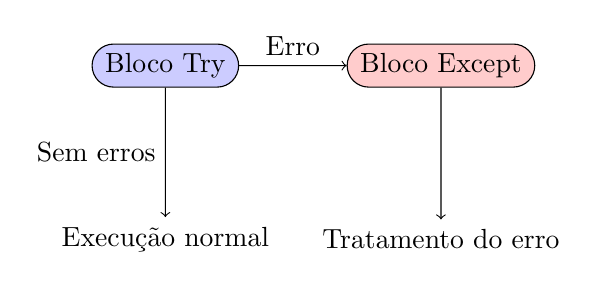
\begin{tikzpicture}[node distance=1.5cm]
            \node (try) [rounded rectangle, draw, fill=blue!20] {Bloco Try};
            \node (except) [rounded rectangle, draw, fill=red!20, right of=try, xshift=2cm] {Bloco Except};
            \node (sucesso) [below of=try, yshift=-0.7cm] {Execução normal};
            \node (falha) [below of=except, yshift=-0.7cm] {Tratamento do erro};

            \draw [->] (try) -- node[left] {Sem erros} (sucesso);
            \draw [->] (try) -- node[above] {Erro} (except);
            \draw [->] (except) -- (falha);
        \end{tikzpicture}
    \end{exampleblock}

    \begin{alertblock}{Como podemos fazer o tratamento?}
        \begin{itemize}
            \item Especificar o tipo de exceção
            \item Registrar que ocorreu um problema
            \item Definir valores padrão caso tenha um problema
        \end{itemize}
    \end{alertblock}
\end{frame}

\begin{frame}[fragile]{Exemplo  de tratamento}
    \begin{block}{Exemplo de tratamento}
        \begin{verbatim}
try:
    print("Início do bloco try")
    x = 10 / 0  # O problema ocorre aqui
    print("Esta linha NUNCA será executada")
except ZeroDivisionError:
    print("Erro capturado - divisão por zero")
\end{verbatim}
    \end{block}




\end{frame}

\begin{frame}[fragile]{Qual problema temos aqui?}
    \begin{block}{Código Vulnerável}
        \begin{verbatim}
idade = int(input("Digite sua idade: "))
if idade >= 18:
    print("Maior de idade")
else:
    print("Menor de idade")
\end{verbatim}
    \end{block}

    \begin{alertblock}{O que pode dar errado?}
        Porque esse código é vulnerável ?
    \end{alertblock}


\end{frame}

\begin{frame}[fragile]{Problema com Entrada do Usuário}
    \begin{block}{Código Vulnerável}
        \begin{verbatim}
idade = int(input("Digite sua idade: "))
if idade >= 18:
    print("Maior de idade")
else:
    print("Menor de idade")
\end{verbatim}
    \end{block}

    \begin{alertblock}{O que pode dar errado?}
        \begin{itemize}
            \item \textcolor{red}{ValueError}: Se usuário digitar "dez" em vez de 10
        \end{itemize}
    \end{alertblock}


\end{frame}

\begin{frame}[fragile]{Solução com Tratamento de Exceções}
    \begin{block}{Código com o tratamento de exceção}
        \begin{verbatim}
try:
    idade = int(input("Digite sua idade: "))
    if idade >= 18:
        print("Maior de idade")
    else:
        print("Menor de idade")
except ValueError:
    print("Por favor, digite apenas números!")
\end{verbatim}
    \end{block}




\end{frame}

\begin{frame}[fragile]{O que pode dar errado neste codigo?}
    \begin{block}{Discutam o código abaixo}
        \begin{verbatim}

num = int(input("Número: "))  
print(f"Resultado: {100 / num}")        

\end{verbatim}
    \end{block}

\end{frame}

\begin{frame}[fragile]{Riscos levantados}
    \begin{block}{Pontos de risco}
        \begin{verbatim}
num = int(input("Número: "))            # Risco 1: Valor não inteiro
print(f"Resultado: {100 / num}")        # Risco 2: Divisão por zero
\end{verbatim}
    \end{block}

    \begin{itemize}
        \item \textcolor{red}{ValueError}:
              \begin{itemize}
                  \item Entradas como "vinte", "a"...
              \end{itemize}

        \item \textcolor{red}{ZeroDivisionError}:
              \begin{itemize}
                  \item Divisão por zero caso num=0
              \end{itemize}
    \end{itemize}
\end{frame}

\begin{frame}[fragile]{Solução de Tratamento}
    \begin{block}{Código com Tratamento de Erros}
        \begin{verbatim}
try:
    num = int(input("Número: "))
    print(f"Resultado: {100 / num}")
except ValueError:
    print("Digite um número inteiro válido!")
except ZeroDivisionError:
    print("Não pode ser zero!")
\end{verbatim}
    \end{block}



    \begin{exampleblock}{Exemplo de Execuções}
        \begin{itemize}
            \item Entrada "10" → Resultado: 10.0
            \item Entrada "0" → "Não pode ser zero!"
            \item Entrada "abc" → "Digite um número inteiro válido!"
        \end{itemize}
    \end{exampleblock}
\end{frame}

\begin{frame}[fragile]{O Bloco \texttt{else} no Tratamento de Exceções}
    \begin{block}{Quando usar?}
        O bloco \texttt{else} executa \textbf{somente se}:
        \begin{itemize}
            \item O bloco \texttt{try} for concluído \textbf{sem erros}
            \item Nenhuma exceção foi levantada
        \end{itemize}
    \end{block}

    \begin{block}{Diferença entre fluxos}
        \begin{verbatim}
try:
    # Código que pode falhar
except MinhaExcecao:
    # Executa SE ocorrer erro
else:
    # Executa SE NÃO ocorrer erro
finally:
    # Executa SEMPRE
\end{verbatim}
    \end{block}


\end{frame}



\begin{frame}{O bloco \texttt{finally}}
    \begin{block}{Características do \texttt{finally}}
        \begin{itemize}
            \item \textcolor{blue}{Sempre executa}, independentemente:
                  \begin{itemize}
                      \item Se ocorrer erro \textbf{ou não}
                      \item Se o erro foi tratado \textbf{ou não}
                      \item Se houve \texttt{return} no bloco
                  \end{itemize}

            \item Uso típico para:
                  \begin{itemize}
                      \item Liberar recursos (arquivos, conexões)
                      \item Fazer limpeza
                      \item Registrar/logging de operações
                  \end{itemize}
        \end{itemize}
    \end{block}


\end{frame}


\begin{frame}[fragile]{Fluxo Try-Except-Finally}
    \begin{exampleblock}{Fluxo de Execução com Tratamento de Exceções com o finally}
        \centering
        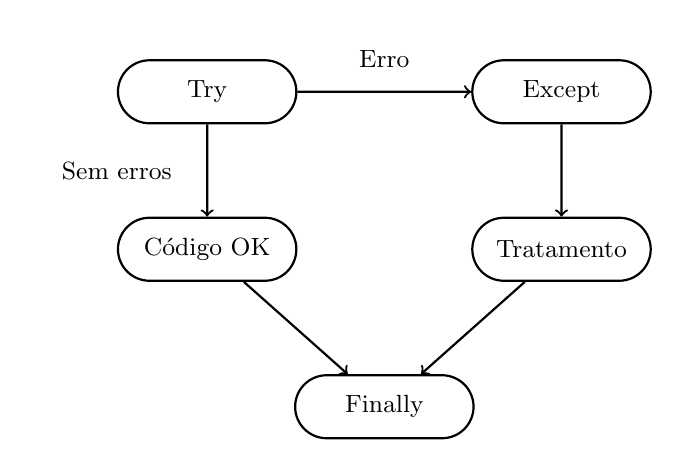
\begin{tikzpicture}[
                every node/.style={
                        rounded rectangle,
                        draw,
                        minimum width=2.5cm,
                        minimum height=0.8cm,
                        align=center,
                        font=\small,
                        fill=white
                    },
                thick
            ]

            % Nós principais posicionados manualmente
            \node (try) at (0, 0) {Try};
            \node (except) at (4.5, 0) {Except};
            \node (sucesso) at (0, -2) {Código OK};
            \node (erro) at (4.5, -2) {Tratamento};
            \node (finally) at (2.25, -4) {Finally};

            % Setas com rótulos sem borda/preenchimento
            \draw[->] (try) -- node[midway, left, draw=none, fill=none, font=\small] {Sem erros} (sucesso);
            \draw[->] (try) -- node[midway, above, draw=none, fill=none, font=\small] {Erro} (except);
            \draw[->] (sucesso) -- (finally);
            \draw[->] (except) -- (erro);
            \draw[->] (erro) -- (finally);

        \end{tikzpicture}
    \end{exampleblock}
\end{frame}

\begin{frame}[fragile]{O Bloco \texttt{finally} em Python}
    \begin{block}{Funcionamento Básico}
        \begin{verbatim}
arquivo = None
try:
    arquivo = open("dados2.txt", "r")
    # Operações com o arquivo
except FileNotFoundError:
    print("Arquivo não encontrado!")
finally:
    print("Sempre executa")
    if arquivo != None:
        arquivo.close()  # Garante o fechamento
    else:
        print(arquivo)
\end{verbatim}
    \end{block}

\end{frame}

\begin{frame}{Hierarquia de Exceções em Python}
    \begin{block}{}
        \small
        Todas as exceções herdam de \texttt{BaseException}. Veja "Exception hierarchy" em \url{https://docs.python.org/3/library/exceptions.html}
    \end{block}

    \begin{center}
        \includegraphics[width=0.8\textwidth]{Images/python_exception_hierarchy.png}
    \end{center}


\end{frame}


\begin{frame}[fragile]{Capturando Exceções Genéricas}
    \begin{block}{Exemplo Prático}
        \begin{verbatim}
try:
    num = int(input("Digite um número: "))
    resultado = 100 / num
    print(f"Resultado: {resultado}")
    
except Exception as err:  
    print(f"Ocorreu um erro: {type(err).__name__}")
    print(f"Mensagem: {str(err)}")
    print(f"Detalhes completo: {err}")
\end{verbatim}
    \end{block}
\end{frame}

\begin{frame}[fragile]{Tratando Diferentes Tipos de Exceções}
    \begin{block}{Exemplo Completo}
        \begin{verbatim}
try:
    num = int(input("Digite um número (não zero): "))
    resultado = 100 / num
    print(f"Resultado: {resultado:.2f}")

except ZeroDivisionError:
    print("Erro: Não é possível dividir por zero!")
except ValueError:
    print("Erro: Digite apenas números inteiros!")

except BaseException as err:
    print()
    print(f"Ops! {type(err).__name__}")
    print(f"Fim!")
\end{verbatim}
    \end{block}

\end{frame}

\begin{frame}[fragile]{Exceções Personalizadas}
    \begin{block}{Como criar uma exceção básica}
        \begin{verbatim}
class MeuErroCustomizado(Exception):
    pass

raise MeuErroCustomizado("Mensagem de erro especial")
\end{verbatim}
    \end{block}

    \begin{exampleblock}{Exemplo Prático}
        \begin{verbatim}
try:
    raise MeuErroCustomizado("Algo deu errado!")
except MeuErroCustomizado as erro:
    print(f"Erro capturado: {erro}")
\end{verbatim}

        \small
        \textbf{Saída:}\\
        \ttfamily
        Erro capturado: Algo deu errado!
    \end{exampleblock}

\end{frame}



\begin{frame}[fragile]{Verificação de Triângulo Equilátero}
    \begin{block}{Código que verifica se os lados formam um triângulo equilátero}
        \begin{verbatim}
def verifica_equilatero(triangulo):
    if triangulo[0] == triangulo[1] == triangulo[2]:
        return True
    else:
        raise ValueError("Não é um triângulo equilátero!")

try:
    lados = [5, 5, 5]  
    if verifica_equilatero(lados):
        print("É um triângulo equilátero!")
except ValueError as e:
    print(f"Erro: {e}")
\end{verbatim}
    \end{block}
\end{frame}

\begin{frame}[fragile]{Exceções - Criando exceções personalizadas}

    \begin{block}{Quando usar?}
        Usada quando precisamos definir nossos próprios tipos de erro para tornar o código mais legível e facilitar o tratamento de erros específicos.
    \end{block}

    \begin{block}{Passo a passo para criação}
        \begin{enumerate}
            \item Criar uma classe que herda de \texttt{Exception}
            \item Definir um construtor (\texttt{\_\_init\_\_}) para personalizar a exceção
            \item Levantar a exceção (\texttt{raise}) no código
            \item Capturar a exceção (\texttt{except}) e tratá-la
        \end{enumerate}
    \end{block}


\end{frame}


\begin{frame}[fragile]{Exceções - Criando exceções personalizadas}

    \begin{block}{1. Criar uma classe que herda de Exception}
        Cada exceção personalizada deve ser uma classe que herda da classe Exception. Isso garante que ela tenha o comportamento de uma exceção normal.
    \end{block}

    \begin{exampleblock}{Exemplo Básico}
        \begin{verbatim}
class SaldoInsuficienteError(Exception):
    """Exceção para indicar que o saldo da conta é insuficiente."""
    pass
\end{verbatim}
    \end{exampleblock}

    \begin{block}{}
        \small
        \texttt{SaldoInsuficienteError} já funciona como uma exceção, mas ainda não tem uma mensagem personalizada.
    \end{block}


\end{frame}

\begin{frame}[fragile]{Exceções - Criando exceções personalizadas}

    \begin{block}{2. Definir um construtor (\texttt{\_\_init\_\_}) para personalizar a exceção}
        Podemos adicionar um construtor para aceitar parâmetros e definir uma mensagem de erro.
    \end{block}

    \begin{exampleblock}{Exemplo com construtor personalizado}
        \begin{verbatim}
class SaldoInsuficienteError(Exception):
    """Exceção para saldo insuficiente."""
    def __init__(self, saldo, valor, 
                 mensagem="Saldo insuficiente para a operação."):
        self.saldo = saldo
        self.valor = valor
        self.mensagem = f"{mensagem} Saldo atual: R${saldo:.2f}, valor 
solicitado: R${valor:.2f}."
        super().__init__(self.mensagem)
\end{verbatim}
    \end{exampleblock}


\end{frame}

\begin{frame}[fragile]{Exceções - Criando exceções personalizadas}

    \begin{block}{3. Levantar a exceção (\texttt{raise}) no código}
        Agora podemos usar \texttt{raise} para lançar essa exceção em uma função.
    \end{block}

    \begin{exampleblock}{Exemplo de uso com \texttt{raise}}
        \begin{verbatim}
def sacar(saldo, valor):
    if valor > saldo:
        raise SaldoInsuficienteError(saldo, valor)
    saldo -= valor
    return saldo
\end{verbatim}
    \end{exampleblock}

\end{frame}


\begin{frame}[fragile]{Exceções - Criando exceções personalizadas}

    \begin{block}{4. Capturar a exceção (\texttt{except}) e tratá-la no código}
        Como qualquer outra exceção, podemos capturá-la com \texttt{try-except}
    \end{block}

    \begin{exampleblock}{Exemplo completo de tratamento}
        \begin{verbatim}
try:
    saldo_atual = 100.0
    novo_saldo = sacar(saldo_atual, 200.0)
    print(f"Saque realizado! Novo saldo: R${novo_saldo:.2f}")
except SaldoInsuficienteError as e:
    print(f"Erro: {e}")
\end{verbatim}
    \end{exampleblock}


\end{frame}

\begin{frame}[fragile]{Criando Exceções Personalizadas}
    \small
    \begin{verbatim}
class SaldoInsuficienteError(Exception):
    def __init__(self, saldo, valor, mensagem="Saldo insuficiente para a 
    operação."):
        self.saldo = saldo
        self.valor = valor
        self.mensagem = f"{mensagem} Saldo atual: R${saldo:.2f}, 
        valor solicitado: R${valor:.2f}."
        super().__init__(self.mensagem)
def sacar(saldo, valor):
    if valor > saldo:
        raise SaldoInsuficienteError(saldo, valor)
    saldo -= valor
    return saldo
try:
    saldo_atual = 100.0
    novo_saldo = sacar(saldo_atual, 20.0)
    print(f"Saque realizado! Novo saldo: R${novo_saldo:.2f}")
except SaldoInsuficienteError as e:
    print(f"Erro: {e}")

\end{verbatim}

\end{frame}

\begin{frame}{Dicas e melhores práticas}
    \begin{itemize}
        \item Não use \textit{except Exception} de forma genérica.
        \item Não use \textit{except} sem nenhuma exceção.
        \item Para pegar uma exceção e tratar, precisa que o código que você queira testar esteja dentro do \textit{try}
        \item Não sabe qual exceção pegar? Leia a documentação do python
              \begin{itemize}
                  \item Google é seu amigo, procure por \textit{"python exception list"}
                  \item ou vá na URL: \url{https://docs.python.org/3/library/exceptions.html}
              \end{itemize}
    \end{itemize}

\end{frame}

%----------------------------------------------------------------------------------------
%    TITLE PAGE
%----------------------------------------------------------------------------------------

\title{Persistência de Dados}

\author{Prof. Gabriel Rodrigues Caldas de Aquino}

\institute
{
    gabrielaquino@ic.ufrj.br\\
    
    Instituto de Computação -
    Universidade Federal do Rio de Janeiro % Your institution for the title page
}
\date{Compilado em: \\ \today} % Date, can be changed to a custom date

%----------------------------------------------------------------------------------------
%    PRESENTATION SLIDES
%----------------------------------------------------------------------------------------

%------------------------------------------------
\section{Persistência de Dados}
%------------------------------------------------

\begin{frame}
    % Print the title page as the first slide
    \titlepage
\end{frame}



\begin{frame}{Persistência de Dados}
    \begin{block}{Problema}
        Os dados gerados em uma execução do código são perdidos quando o programa é encerrado.
    \end{block}
    
    \begin{block}{Solução}
        Se precisamos usar os dados no futuro, é necessário armazená-los de forma persistente.
    \end{block}
    
    \vspace{0.5cm}
    
    \textbf{Mecanismos de Persistência de Dados:}
    \begin{itemize}
        \item Arquivos (TXT, CSV, JSON, XML)
        \item Bancos de dados (SQLite, PostgreSQL, MySQL)
    \end{itemize}
\end{frame}

\begin{frame}{Persistência em Arquivos de Texto}
    \begin{block}{Características}
        \begin{itemize}
            \item Formatos comuns: \texttt{.txt}, \texttt{.csv}, \texttt{.json}
            \item Armazenamento disco rígido
            \item Manipulação via objetos da classe \texttt{File}
        \end{itemize}
    \end{block}
    
    \begin{exampleblock}{Para manipular temos um "protocolo" de Uso}
        Três etapas: \textbf{Abrir}, \textbf{Manipular} e \textbf{Fechar}

    \end{exampleblock}
    
\end{frame}

\begin{frame}{Fluxo para se fazer a manipulação de arquivos}
    \centering
    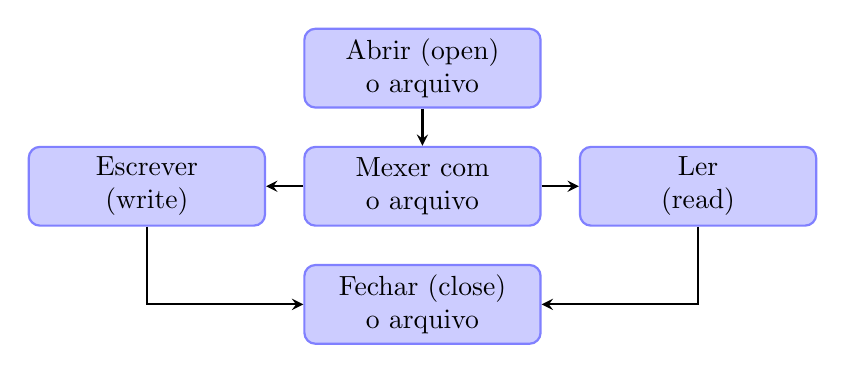
\begin{tikzpicture}[
        node distance=1.5cm,
        etapa/.style={
            rectangle,
            rounded corners,
            draw=blue!50,
            fill=blue!20,
            thick,
            minimum width=3cm,
            minimum height=1cm,
            align=center
        },
        arrow/.style={->, >=stealth, thick}
    ]
    
    \node[etapa] (abrir) {Abrir (open) \\ o arquivo};
    \node[etapa, below of=abrir] (mexer) {Mexer com \\ o arquivo};
    \node[etapa, left of=mexer, xshift=-2cm] (escrever) {Escrever \\ (write)};
    \node[etapa, right of=mexer, xshift=2cm] (ler) {Ler \\ (read)};
    \node[etapa, below of=mexer] (fechar) {Fechar (close) \\ o arquivo};
    
    \draw[arrow] (abrir) -- (mexer);
    \draw[arrow] (mexer) -- (escrever);
    \draw[arrow] (mexer) -- (ler);
    \draw[arrow] (escrever) |- (fechar);
    \draw[arrow] (ler) |- (fechar);
    
    \end{tikzpicture}

    
   
\end{frame}


\begin{frame}[fragile]{Abrindo Arquivos em Python}
    \begin{block}{Método \texttt{open()}}
        Usado para abrir um arquivo. Requer dois parâmetros principais:
\begin{verbatim}
    arquivo = open("nome_do_arquivo.txt", "modo_de_abertura")
\end{verbatim}
        
    \end{block}
    
    \begin{columns}[T]
        \begin{column}{0.5\textwidth}
            \begin{exampleblock}{Parâmetros}
                \begin{itemize}
                    \item \textbf{Nome do arquivo}: \begin{itemize}
                        \item Caminho completo ou relativo
                    \end{itemize}
                    \item \textbf{Modo de abertura}:
                    \begin{itemize}
                        \item \texttt{"r"} - Leitura 
                        \item \texttt{"w"} - Escrita 
                    \end{itemize}
                \end{itemize}
            \end{exampleblock}
        \end{column}
        
        \begin{column}{0.5\textwidth}
            \begin{alertblock}{Exemplos}
\begin{verbatim}
   
# Para escrita
arq = open("dados.txt", "w")

# Para leitura
arq = open("dados.txt", "r")

\end{verbatim}
            \end{alertblock}
        \end{column}
    \end{columns}
    
    \vspace{0.3cm}
    

\end{frame}
\begin{frame}{Modos de Abertura de Arquivos}
    \begin{block}{}
        O modo de abertura define como interagiremos com o arquivo:
    \end{block}

    \centering
    \begin{tabular}{|l|l|l|}
        \hline
        \textbf{Modo} & \textbf{Descrição} & \textbf{Existência do Arquivo} \\
        \hline
        \texttt{r} & Leitura apenas & Deve existir \\
        \hline
        \texttt{w} & Escrita & Cria se não existir \\
        \hline
        \texttt{a} & Escrita no final & Cria se não existir \\
        \hline
        \texttt{r+} & Leitura e escrita & Deve existir \\
        \hline
        \texttt{w+} & Leitura e escrita  & Cria se não existir \\
        \hline
        \texttt{a+} & Leitura e escrita no final & Cria se não existir \\
        \hline
    \end{tabular}
    
\end{frame}


\begin{frame}{Modos de Abertura de Arquivo}

\centering
\includegraphics[width=0.8\textwidth]{Images/diagrama-modos-leitura.png}


\end{frame}


\begin{frame}[fragile]{Abrindo Arquivos - Modo de abertura 'r'}
\begin{itemize}
    \item Método read: ler dados de um arquivo que foi previamente aberto para leitura
    \item Para abrir um arquivo para leitura: 
    \begin{itemize}
        \item Precisamos dar o nome de um arquivo existente 
        \item Em seguida indicar o modo de leitura \textit{r} no momento da abertura
    \end{itemize}

\end{itemize}

\begin{block}{Abrindo o arquivo dados.txt}
\begin{verbatim}
arquivo = open("dados.txt", "r")
conteudo = arquivo.read()
print(conteudo)
arquivo.close()
\end{verbatim}
\end{block}

\end{frame}



\begin{frame}[fragile]{Lendo linha por linha}

\begin{itemize}
    \item Em arquivos com múltiplas linhas podemos usar for loop para facilitar o tratamento linha por linha
\end{itemize}
    
\begin{exampleblock}{Exemplo de leitura linha por linha}
\begin{verbatim}
arquivo="dados.txt"
arq = open(arquivo, "r")
numero_da_linha = 1
for linha in arq:
    print(f"Linha {numero_da_linha}: {linha}")
    numero_da_linha = numero_da_linha + 1
arq.close()
\end{verbatim}
\end{exampleblock}


\end{frame}

\begin{frame}[fragile]{Escrever em Arquivo: write() - Modo de abertura 'w'}

\begin{block}{Método write()}
\begin{verbatim}
arq.write("conteúdo que será escrito no arquivo")
\end{verbatim}
\end{block}

\begin{block}{Passos para escrita em arquivo}
\begin{enumerate}
\item Abrir o arquivo em modo de escrita (\texttt{'w'})
\item Passar o conteúdo como string para \texttt{write()}
\item Fechar o arquivo
\end{enumerate}
\end{block}

\end{frame}

\begin{frame}[fragile]{Escrita Básica em Arquivos}
\begin{block}{Exemplo de escrita em arquivo}
\begin{verbatim}
arq = open("nomes.txt", "w")
arq.write("Gabriel, Pedro, Manoel")
arq.close()
\end{verbatim}
\end{block}

\begin{block}{Importante!}
\begin{itemize}
\item \texttt{'w'} = write (escrita)
\item Sempre feche o arquivo após escrever
\item Cada \texttt{write()} grava o conteúdo exato
\item Se o arquivo "nomes.txt" \textbf{já existe}, ele será \textbf{sobrescrito}
\end{itemize}
\end{block}
\end{frame}

\begin{frame}[fragile]{Arquivos com mais de uma linha}

\begin{block}{Leitura de Arquivos Linha por Linha}
\begin{itemize}
    \item Arquivos com múltiplas linhas contêm \texttt{\textbackslash n} escondido

\end{itemize}
\end{block}

\begin{exampleblock}{Exemplo Prático}
Pedro\textbackslash n

Antonio\textbackslash n

Maria\textbackslash n

Jose\textbackslash n
\end{exampleblock}

\end{frame}

\begin{frame}[fragile]{Pulando linha na escrita em arquivos}

\begin{block}{Código de exemplo}
\begin{verbatim}
arq = open("nomes.txt", "w")
arq.write("Gabriel\nPedro\nManoel")
arq.close()
\end{verbatim}
\end{block}



\begin{alertblock}{O que acontece?}
\begin{itemize}
\item \texttt{\textbackslash n} é o \textbf{caractere especial} para quebra de linha
\item Quando escrito no arquivo, ele:
  \begin{itemize}
  \item Finaliza a linha atual
  \item Move o cursor para a próxima linha
  \end{itemize}

\end{itemize}
\end{alertblock}


\end{frame}

\begin{frame}[fragile]{Fechando o Arquivo: close()}

\begin{block}{Método close()}
\begin{verbatim}
arq.close()  # Fecha o arquivo após uso
\end{verbatim}
\end{block}

\begin{alertblock}{Por que fechar arquivos?}
\begin{itemize}
\item \textbf{Libera recursos do sistema}: Arquivos abertos consomem memória
\item \textbf{Garante a escrita completa}: Dados podem ficar em buffer
\item \textbf{Evita corrupção}: Previne acesso concorrente indevido
\item \textbf{Libera o arquivo}: Permite que outros programas o acessem
\end{itemize}
\end{alertblock}


\end{frame}


\begin{frame}[fragile]{Modo de Abertura 'a' (Append)}
    \begin{block}{Funcionamento do modo \texttt{"a"}}
        \begin{verbatim}
arquivo = open("dados.txt", "a")  # Modo append
arquivo.write("Novo conteúdo\n")
arquivo.close()
        \end{verbatim}
    \end{block}

            \begin{alertblock}{Características}
                \begin{itemize}
                    \item \textbf{Abre para escrita} no final do arquivo
                    
                    \item Ponteiro no \textbf{fim do arquivo} (só escreve no final)
                \end{itemize}
            \end{alertblock}

        

\end{frame}


\begin{frame}[fragile]{Gerenciamento de Arquivos com \texttt{with open}}
    \begin{block}{Sintaxe Básica}
        \begin{verbatim}
with open("arquivo.txt", "modo") as arquivo:
    # Bloco de código
        \end{verbatim}
    \end{block}

            \begin{exampleblock}{Exemplo Prático}
                \begin{verbatim}
with open("dados.txt", "r") as arq:
    conteudo = arq.read()
    print(conteudo)
                \end{verbatim}
            \end{exampleblock}
   

    \begin{block}{Facilidade}
    \begin{itemize}
        \item O \texttt{with} deixa arquivo aberto.
        \item Ao sair do bloco, o \texttt{close()} é  automático.
    \end{itemize}
         
    \end{block}
\end{frame}

\begin{frame}[fragile]{Controlando a Posição com \texttt{seek()}}

    \begin{block}{O que é \texttt{seek()}?}
        Método que permite mover o "cursor" de leitura/escrita para qualquer posição no arquivo
        \begin{verbatim}
arquivo.seek(offset)
        \end{verbatim}
    \end{block}

  
            \begin{alertblock}{Parâmetros}
                \begin{itemize}
                    \item \textbf{offset}: Número de bytes para mover
                    
                \end{itemize}
            \end{alertblock}
      
            \begin{exampleblock}{Exemplos}
                \begin{verbatim}
# Ir para o byte 10
arquivo.seek(10)
                \end{verbatim}
            \end{exampleblock}
 


    
   
\end{frame}

\begin{frame}[fragile]{Modo de Abertura \texttt{r+}}

\begin{block}{Funcionamento do modo \texttt{"r+"}}
\begin{verbatim}
with open("arquivo.txt", "r+") as arquivo:
    # Operações de leitura E escrita
    conteudo = arquivo.read()  # Lê
    arquivo.write("novo texto")  # Escreve
\end{verbatim}
\end{block}

        \begin{alertblock}{Características}
            \begin{itemize}
                \item Permite \textbf{leitura e escrita} no mesmo arquivo
               \item Não apaga o arquivo na hora de abrir
                \item Posição inicial: \textbf{início do arquivo}
            \end{itemize}
        \end{alertblock}

\end{frame}

\begin{frame}[fragile]{Modo de Abertura \texttt{w+} (Escrita e Leitura)}
    \begin{block}{Funcionamento do modo \texttt{"w+"}}
        \begin{verbatim}
with open("arquivo.txt", "w+") as arquivo:
    arquivo.write("Conteúdo inicial\n")
    arquivo.seek(0)  # Volta ao início para leitura
    conteudo = arquivo.read()
    print(conteudo)
        \end{verbatim}
    \end{block}

    \begin{columns}[T]
        \begin{column}{0.5\textwidth}
            \begin{alertblock}{Características Principais}
                \begin{itemize}
                    \item \textbf{Apaga conteúdo existente}
                   
                    \item Posição inicial: \textbf{início do arquivo}
                    
                \end{itemize}
            \end{alertblock}
        \end{column}
        
        \begin{column}{0.5\textwidth}
            
            
            \begin{block}{Cuidado!}
                Sempre use \texttt{seek()} antes de ler após escrever
            \end{block}
        \end{column}
    \end{columns}


\end{frame}
\begin{frame}[fragile]{Modo de Abertura \texttt{a+} (Append e Leitura)}

\begin{block}{Funcionamento do modo \texttt{"a+"}}
\begin{verbatim}
with open("arquivo-teste.txt", "a+") as arquivo:
    arquivo.write("Nova entrada\n")  # Escreve no FINAL
    arquivo.seek(0)                  # Volta ao início
    texto = arquivo.read()       # Lê todo conteúdo
    print(texto)
\end{verbatim}
\end{block}

        \begin{alertblock}{Características}
            \begin{itemize}
               \item \textbf{Não apaga} conteúdo existente 
               \item Posição inicial:  \textbf{Final do arquivo}
                
            \end{itemize}
        \end{alertblock}
\end{frame}




\begin{frame}[fragile]{Tratamento de Exceções com Arquivos}

\begin{block}{Por que tratar exceções?}
Lidar com arquivos pode lançar exceções inesperadas que devem ser gerenciadas.
\end{block}

\begin{block}{Principais exceções com arquivos}
\begin{itemize}
\item \texttt{FileNotFoundError}: Arquivo não existe ou caminho incorreto
\item \texttt{IOError}: Erros gerais de entrada/saída (disco cheio, permissões)
\end{itemize}
\end{block}




\end{frame}

\begin{frame}[fragile]{Tratamento de Exceções com Arquivos}

\begin{block}{Código de Exemplo}
\begin{verbatim}
try:
    f = open("arquivo-inexistente.txt", "r")
    conteudo = f.read()
    f.close()
    print(conteudo)
except FileNotFoundError:
    print("Arquivo não existente")
\end{verbatim}
\end{block}




\end{frame}

\begin{frame}[fragile]{Demonstração: Tratando Arquivo Corrompido}

\begin{block}{Código de Tratamento}
\begin{verbatim}
try:
    f = open("arquivo-corrompido.txt", "r")
    conteudo = f.read()
    f.close()
    print(conteudo)
except IOError:
    print("Erro: Problema ao ler o arquivo")
\end{verbatim}
\end{block}


\end{frame}


%----------------------------------------------------------------------------------------
%    TITLE PAGE
%----------------------------------------------------------------------------------------

\title{Biblioteca Numpy}

\author{Prof. Gabriel Rodrigues Caldas de Aquino}

\institute
{
    gabrielaquino@ic.ufrj.br\\
    
    Instituto de Computação -
    Universidade Federal do Rio de Janeiro % Your institution for the title page
}
\date{03 de Junho de 2025} % Date, can be changed to a custom date

%----------------------------------------------------------------------------------------
%    PRESENTATION SLIDES
%----------------------------------------------------------------------------------------


\begin{frame}
    % Print the title page as the first slide
    \titlepage
\end{frame}

%------------------------------------------------
\section{Sobre o numpy}
%------------------------------------------------

\begin{frame}{NumPy - Introdução}

\begin{block}{O que é NumPy?}
\begin{itemize}
    \item Pacote fundamental para \textbf{computação científica} em Python
   
    
\end{itemize}
\end{block}

\begin{block}{Objeto principal: \texttt{numpy.ndarray}}
\begin{itemize}
    \item Vetor \textbf{n-dimensional} (arrays multidimensionais)
    \item Características fundamentais:
    \begin{itemize}
        \item \textbf{Tamanho fixo} (definido na criação)
        \item \textbf{Indexado} por tuplas de inteiros positivos
        \item \textbf{Homogêneo} - todos elementos do mesmo tipo
    \end{itemize}
\end{itemize}
\end{block}

\begin{exampleblock}{Documentação Oficial}
\centering

Há diversas métodos e atributos disponíveis no NumPy, os quais podem ser consultados na documentação oficial no endereço:
\url{https://numpy.org/doc/stable/index.html}


\end{exampleblock}


\end{frame}

\begin{frame}[fragile]{NumPy - Arrays}

\begin{block}{Importe o módulo e crie arrays a partir de listas}

    \begin{verbatim}
    import numpy as np
    np.array(lista)
    \end{verbatim}

\end{block}
\begin{columns}[T]
    \begin{column}{0.5\textwidth}
\begin{exampleblock}{Exemplos}
\begin{verbatim}
# Array 1D (vetor)
x = np.array([1, 2, 3])


# Array 2D (matriz)
y = np.array([[1., 0., 0.], 
              [0., 1., 0.]])

\end{verbatim}
\end{exampleblock}
    \end{column}
    
  \begin{column}{0.5\textwidth}  
  \begin{block}{Saída dos Exemplos}
        \begin{verbatim}
#Saída:
>>> x
array([1, 2, 3])

>>> y
array([[1., 0., 0.],
       [0., 1., 0.]])
 \end{verbatim}
        \end{block}
    \end{column}
\end{columns} 
\end{frame}

\begin{frame}{Tipos de Numpy array}

\begin{alertblock}{Verificando o Tipo}
        \begin{verbatim}

>>> type(x)
numpy.ndarray

>>> type(y)
numpy.ndarray
        \end{verbatim}
\end{alertblock}


\begin{block}{Características}
\begin{itemize}
    \item \texttt{x} é um array \textbf{1-dimensional} (vetor)
    \item \texttt{y} é um array \textbf{2-dimensional} (matriz)
    \item Ambos são do tipo \texttt{numpy.ndarray}
\end{itemize}
\end{block}
\end{frame}

\begin{frame}[fragile]{NumPy - O Atributo \texttt{dtype}}

\begin{block}{Definição}
O \texttt{dtype} define o tipo dos elementos armazenados no array NumPy
\end{block}

\begin{exampleblock}{Exemplo Inicial}
\begin{verbatim}
minhalista = [1, 2, 3, 4, 5]
arr = np.array(minhalista)
print(arr)          # array([1, 2, 3, 4, 5])
print(type(arr))    # <class 'numpy.ndarray'>
print(arr.dtype)    # dtype('int64')
\end{verbatim}
\end{exampleblock}

\begin{columns}[T]
    \begin{column}{0.5\textwidth}
        \begin{alertblock}{Com Número Decimal}
\begin{verbatim}
minhalista = [1, 2, 3, 4, 5.5]
arr = np.array(minhalista)
print(arr.dtype)  # dtype('float64')
\end{verbatim}
        \end{alertblock}
    \end{column}
    
    \begin{column}{0.5\textwidth}
        \begin{alertblock}{Com String}
\begin{verbatim}
minhalista = [1, 2, 3, 4, "ola"]
arr = np.array(minhalista)
print(arr.dtype)  # dtype('<U21')
\end{verbatim}
        \end{alertblock}
    \end{column}
\end{columns}


\end{frame}



%----------------------------------------------------------------------------------------
%    TITLE PAGE
%----------------------------------------------------------------------------------------

\title{Biblioteca Matplotlib}

\author{Prof. Gabriel Rodrigues Caldas de Aquino}

\institute
{
    gabrielaquino@ic.ufrj.br\\
    
    Instituto de Computação -
    Universidade Federal do Rio de Janeiro % Your institution for the title page
}
\date{Compilado em: \\ \today} % Date, can be changed to a custom date

%----------------------------------------------------------------------------------------
%    PRESENTATION SLIDES
%----------------------------------------------------------------------------------------

%------------------------------------------------
\section{Biblioteca Matplotlib}
%------------------------------------------------

\begin{frame}
    % Print the title page as the first slide
    \titlepage
\end{frame}



\begin{frame}{Origem e Popularidade do \texttt{Matplotlib}}
    \begin{itemize}
        \item Criado por John D. Hunter em 2003 como uma biblioteca de gráficos em Python.
        \item Inspirado no \texttt{MATLAB}, com o objetivo de permitir a criação de visualizações de alta qualidade por cientistas e engenheiros.
        \item Atualmente, é amplamente utilizado em áreas como:
        \begin{itemize}
            \item Ciência de dados,
            \item Engenharia,
            \item Aprendizado de máquina.
        \end{itemize}
    \end{itemize}
\end{frame}

\begin{frame}{Para que Serve o \texttt{Matplotlib}?}
    \begin{itemize}
        \item O \texttt{matplotlib} é usado para:
        \begin{itemize}
            \item Criar gráficos e visualizações de dados em Python.
            \item Analisar visualmente comportamentos, tendências e padrões.
            \item Produzir figuras de alta qualidade para relatórios, artigos e apresentações.
        \end{itemize}

        \item Com ele, é possível gerar:
        \begin{itemize}
            \item Gráficos de linha, barra, pizza, dispersão (scatter), histogramas, entre outros.
        \end{itemize}

        \item É uma ferramenta essencial em:
        \begin{itemize}
            \item Ciência de dados,
            \item Engenharia,
            \item Pesquisa científica,
            \item Educação.
        \end{itemize}
    \end{itemize}
\end{frame}


\begin{frame}{Introdução ao \texttt{pyplot}}
    \begin{itemize}
        \item \texttt{matplotlib.pyplot} é uma coleção de funções que faz o \texttt{matplotlib} funcionar de forma semelhante ao \texttt{MATLAB}.
        \item Cada função do \texttt{pyplot} realiza uma alteração na figura: cria uma figura, define uma área de plotagem, desenha linhas, adiciona rótulos, etc.
        \item O \texttt{pyplot} mantém estados entre chamadas de função, acompanhando a figura e a área de plotagem atual.
        \item \textbf{Axes} são componentes centrais da figura.
    \end{itemize}
\end{frame}



\begin{frame}[fragile]{Criando Visualizações com \texttt{pyplot}}
    \begin{itemize}
        \item Gerar visualizações com \texttt{pyplot} é rápido e simples.
        \item Exemplo básico:
    \end{itemize}

    \begin{block}{Exemplo em Python}
    \begin{verbatim}
import matplotlib.pyplot as plt

plt.plot([1, 2, 3, 4])
plt.ylabel('alguns números')
plt.title('Titulo')
plt.show()
    \end{verbatim}
    \end{block}
\end{frame}

\begin{frame}{Explicação do Código}
    \begin{itemize}
        \item \texttt{import matplotlib.pyplot as plt} \\
        Importa a biblioteca \texttt{pyplot} do \texttt{matplotlib}  como \texttt{plt} para facilitar o uso.
        \item \texttt{plt.plot([1, 2, 3, 4])} \\
        Cria um gráfico de linha simples com os valores fornecidos no eixo y;\\ O eixo x é automático (índices 0 a 3).
        \item \texttt{plt.ylabel('alguns números')} \\
        Define o rótulo do eixo y com o texto "alguns números".
        \item \texttt{plt.title('Titulo')} \\
        Adiciona um título ao gráfico.
        \item \texttt{plt.show()} \\
        Exibe a figura gerada em uma janela ou no ambiente gráfico.
    \end{itemize}
\end{frame}


\begin{frame}[fragile]{Plotando x versus y com \texttt{pyplot}}
    Para plotar valores de x contra y, você pode modificar o código anterior assim:

    \begin{block}{Exemplo em Python}
\begin{verbatim}
import matplotlib.pyplot as plt

plt.plot([1, 2, 3, 4], [1, 4, 9, 16])
plt.xlabel('valores de x')
plt.ylabel('alguns números')
plt.show()
\end{verbatim}
    \end{block}
\end{frame}

\begin{frame}[fragile]{Adicionando Anotações com \texttt{plt.annotate()}}
    \begin{itemize}
        \item O método \texttt{plt.annotate()} permite destacar pontos importantes no gráfico com texto e setas.
        \item Parâmetros usados:
        \begin{itemize}
            \item \texttt{xy=(2, 4)}: coordenada do ponto a ser anotado.
            \item \texttt{xytext=(3, 6)}: posição do texto da anotação.
            \item \texttt{arrowprops}: define propriedades da seta (ex: cor).
        \end{itemize}
    \end{itemize}

    \begin{block}{Exemplo em Python}
\begin{verbatim}
import matplotlib.pyplot as plt

plt.plot([1, 2, 3], [1, 4, 9])
plt.annotate('ponto importante', xy=(2, 4),
             xytext=(3, 6),
             arrowprops=dict(facecolor='black'))
plt.show()
\end{verbatim}
    \end{block}
\end{frame}


\begin{frame}[fragile]{Exemplo de Marcadores e Estilo de Linha em \texttt{pyplot}}
    \begin{itemize}
        \item O parâmetro \texttt{markersize} ajusta o tamanho dos marcadores nos pontos do gráfico.
        \item O estilo \texttt{'ko:'} significa:
        \begin{itemize}
            \item \texttt{k}: cor preta (black).
            \item \texttt{o}: marcador circular.
            \item \texttt{:}: linha pontilhada.
        \end{itemize}
    \end{itemize}

    \begin{block}{Exemplo em Python}
\begin{verbatim}
import matplotlib.pyplot as plt

plt.plot([2, 1], [3, 1], 'ko:', markersize=10)
plt.xlabel('x')
plt.ylabel('y')
plt.show()
\end{verbatim}
    \end{block}
\begin{itemize}
    \item  \url{https://matplotlib.org/stable/api/_as_gen/matplotlib.pyplot.plot.html}
\end{itemize}
\end{frame}

\begin{frame}[fragile]{Adicionando Grid ao Gráfico}
    \begin{itemize}
        \item O método \texttt{plt.grid(True)} adiciona uma grade (grid) ao gráfico, facilitando a leitura dos valores.
        \item É especialmente útil para visualizações com muitos dados ou comparações visuais.
    \end{itemize}

    \begin{block}{Exemplo em Python}
\begin{verbatim}
import matplotlib.pyplot as plt

plt.plot([1, 2, 3, 4], [1, 4, 9, 16], 'bo-')
plt.xlabel('x')
plt.ylabel('y')
plt.grid(True)
plt.show()
\end{verbatim}
    \end{block}
\end{frame}

\begin{frame}[fragile]{Definindo os Limites dos Eixos com \texttt{plt.axis}}
    \begin{itemize}
        \item O método \texttt{plt.axis()} permite definir manualmente os limites dos eixos do gráfico.
        \item A sintaxe \texttt{plt.axis((xmin, xmax, ymin, ymax))} define:
        \begin{itemize}
            \item \texttt{xmin = 0}, \texttt{xmax = 6}
            \item \texttt{ymin = 0}, \texttt{ymax = 20}
        \end{itemize}
        \item Isso pode ser útil para controlar o zoom do gráfico ou garantir uma escala fixa.
    \end{itemize}

    \begin{block}{Exemplo em Python}
\begin{verbatim}
import matplotlib.pyplot as plt

plt.plot([1, 2, 3, 4], [1, 4, 9, 16], 'ro-')
plt.axis((0, 6, 0, 20))
plt.grid(True)
plt.show()
\end{verbatim}
    \end{block}
\end{frame}

\begin{frame}{Gráfico do crescimento populacional}

Vá na página da Wikipédia que contém dados reais de crescimento populacional mundial  \url{https://pt.wikipedia.org/wiki/Crescimento_populacional} e crie um gráfico com o crescimento populacional ao longo dos anos

    
\end{frame}


\begin{frame}[fragile]{Evitando Notação Científica no Eixo Y}
    \begin{itemize}
        \item Quando os valores do eixo Y são muito grandes, o \texttt{matplotlib} ativa a notação científica automaticamente (ex: \texttt{1e6}).
        \item Para desativar essa notação e mostrar os números completos, usamos:
        \begin{itemize}
            \item \texttt{plt.ticklabel\_format(style='plain', axis='y')}
        \end{itemize}
        
    \end{itemize}

    \begin{block}{Exemplo em Python}
\begin{verbatim}
ano = [1750, 1800, 1850, 1900, 1950, 1955, 1960, 1965,
       1970, 1975, 1980, 1985, 1990, 1995, 2000, 2005]
populacao = [791000, 978000, 1262000, 1650000, 2518629,
             2755823, 3021475, 3334874, 3692492, 4063587,
             4434682, 4830979, 5263593, 5674380, 6070581, 6453628]
plt.plot(ano, populacao)
plt.ticklabel_format(style='plain', axis='y')  
plt.show()
\end{verbatim}
    \end{block}
\end{frame}



\begin{frame}[fragile]{Gráfico de Barras: Crescimento Populacional}
    \begin{itemize}
        \item Podemos usar \texttt{plt.bar()} para representar os dados como um gráfico de barras.
        \item Útil para destacar visualmente a variação entre os anos.
    \end{itemize}

    \begin{block}{Exemplo com \texttt{plt.bar()}}
\begin{verbatim}
plt.bar(ano, populacao)
plt.xlabel('Ano')
plt.ylabel('População')
plt.ticklabel_format(style='plain', axis='y')
plt.grid(True)
plt.title('Crescimento Populacional Mundial')
plt.show()
\end{verbatim}
    \end{block}
\end{frame}

\begin{frame}[fragile]{Gráfico de Barras - Tamanho das barras}
    \begin{itemize}
        \item Podemos usar \texttt{plt.bar()} para representar os dados como um gráfico de barras.
        \item O parâmetro \texttt{width} controla a largura das barras.
    \end{itemize}

    \begin{block}{Exemplo com \texttt{plt.bar(..., width=20)}}
\begin{verbatim}

plt.bar(ano, populacao, width=20)
...
plt.show()
\end{verbatim}
    \end{block}
\end{frame}

\begin{frame}[fragile]{\texttt{plot()} vs \texttt{scatter()}}
    \begin{itemize}
        \item Tanto \texttt{plt.plot(..., marker='o')} quanto \texttt{plt.scatter(...)} podem ser usados para representar pontos.
        \item \texttt{plot()} com marcador desenha uma linha conectando os pontos (a menos que especificado para não fazê-lo).
        \item \texttt{scatter()} desenha apenas os pontos individuais, sem conectá-los.
        \item \texttt{scatter()} também permite personalizar tamanho, cor e transparência ponto a ponto.
    \end{itemize}

    \begin{block}{Exemplo em Python}
\begin{verbatim}
a = np.array([0, 2, 4, 0, 2, 2, 3, 2])
b = np.array([0, 1, 0, 0, 0, 2, 1, 1.2])

plt.scatter(a, b, marker='o')  # ou plt.plot(a, b)
plt.grid(True)
plt.show()
\end{verbatim}
    \end{block}
\end{frame}

\begin{frame}[fragile]{Plotando Múltiplas Curvas}
    \begin{itemize}
        \item Podemos usar \texttt{plt.plot()} várias vezes para desenhar múltiplas curvas no mesmo gráfico.
        \item Cada chamada adiciona uma nova série de dados com estilo independente.
    \end{itemize}

    \begin{block}{Exemplo em Python}
\begin{verbatim}
import matplotlib.pyplot as plt

plt.plot([1, 2, 3, 4], [1, 4, 9, 16], 'bo-', label='y = x²')
plt.plot([1, 2, 3, 4], [1, 2, 3, 4], 'rs--', label='y = x')

plt.xlabel('x')
plt.ylabel('y')
plt.grid(True)
plt.legend()
plt.show()
\end{verbatim}
    \end{block}
\end{frame}

\begin{frame}[fragile]{Posicionando a Legenda com \texttt{loc}}
    \begin{itemize}
        \item Use o parâmetro \texttt{loc} para escolher onde a legenda aparece.
        \item Exemplo simples:
    \end{itemize}

    \begin{block}{Código Exemplo}
\begin{verbatim}
import matplotlib.pyplot as plt

plt.plot([1, 2, 3], label='Linha 1')
plt.plot([3, 2, 1], label='Linha 2')

plt.legend(loc='upper right')  # legenda no canto superior direito
plt.show()
\end{verbatim}
    \end{block}
\end{frame}

\begin{frame}{Opções de Localização da Legenda (\texttt{loc})}
    \begin{itemize}
        \item A posição da legenda pode ser controlada com o parâmetro \texttt{loc} da função \texttt{plt.legend()}.
        \item A tabela abaixo mostra 5 posições comuns:
    \end{itemize}

    \vspace{0.5em}
    \begin{table}[]
    \centering
    \begin{tabular}{|c|l|}
        \hline
        \textbf{Código}         & \textbf{Descrição}              \\ \hline
        \texttt{'upper right'}  & Canto superior direito          \\ \hline
        \texttt{'upper left'}   & Canto superior esquerdo         \\ \hline
        \texttt{'lower left'}   & Canto inferior esquerdo         \\ \hline
        \texttt{'lower right'}  & Canto inferior direito          \\ \hline
        \texttt{'center'}       & Centro da área de plotagem      \\ \hline
    \end{tabular}
    \end{table}

    \vspace{0.5em}
    \begin{itemize}
        \item Também é possível usar \texttt{loc='best'} para posicionamento automático.
    \end{itemize}
\end{frame}


\begin{frame}[fragile]{Plotando com \texttt{np.linspace} e \texttt{np.zeros\_like}}
    \begin{itemize}
        \item \texttt{np.linspace(0, 2, 100)} cria 100 pontos igualmente espaçados entre 0 e 2.
        \item \texttt{np.zeros\_like(x)} gera um array de zeros com o mesmo formato de \texttt{x}.
        \item Podemos usar ambos para construir múltiplas curvas no mesmo gráfico.
    \end{itemize}

    \begin{block}{Exemplo em Python}
\begin{verbatim}
import numpy as np
import matplotlib.pyplot as plt

x = np.linspace(0, 2, 100)
y = np.zeros_like(x)

plt.plot(x, y, 'g-')
plt.xlabel('x')
plt.ylabel('y')
plt.grid(True)
plt.show()
\end{verbatim}
    \end{block}
\end{frame}

\begin{frame}[fragile]{Mais de uma curva}
    \begin{itemize}
        \item Podemos construir múltiplas curvas no mesmo gráfico.
    \end{itemize}

    \begin{block}{Exemplo em Python}
\begin{verbatim}
import numpy as np
import matplotlib.pyplot as plt

x = np.linspace(0, 2, 100)
y1 = x**2
y2 = np.zeros_like(x)
plt.plot(x, y1, 'g-', label='y = x²')
plt.plot(x, y2, 'r--', label='y = 0')
plt.xlabel('x')
plt.ylabel('y')
plt.grid(True)
plt.legend()
plt.show()
\end{verbatim}
    \end{block}
\end{frame}

\begin{frame}[fragile]{Cuidado com a Escala dos Dados}
    \begin{itemize}
        \item Funções com crescimento rápido (como \texttt{x\^{}20}) .. (ou também outros dados) .. podem gerar distorções visuais ou comprimir outras curvas.
        \item No exemplo abaixo, a curva \texttt{y = x²} fica quase invisível perto de \texttt{y = x\^{}20}.
    \end{itemize}

    \begin{block}{Exemplo em Python}
\begin{verbatim}
x = np.linspace(-2, 2, 100)
y1 = x**2
y2 = x**20
plt.plot(x, y1, 'g-', label='y = x²')
plt.plot(x, y2, 'r--', label='y = x^20')
plt.xlabel('x')
plt.ylabel('y')
plt.ticklabel_format(style='plain', axis='y')
plt.grid(True)
plt.legend()
plt.show()
\end{verbatim}
    \end{block}
\end{frame}

\begin{frame}[fragile]{Cuidado com o Recorte da Visualização}
    \begin{itemize}
        \item Agora, considere o seguinte trecho: \texttt{plt.axis((-2, 2, 0, 4))}
        
        \item \alert{Pergunta: O que acontece com a curva \texttt{y = x\^{}20} ao aplicar esse recorte?}
    \end{itemize}

    \begin{block}{Código de exemplo}
\begin{verbatim}
x = np.linspace(-2, 2, 100)
y1 = x**2
y2 = x**20
plt.plot(x, y1, 'g-', label='y = x²')
plt.plot(x, y2, 'r--', label='y = x^20')
plt.xlabel('x')
plt.ylabel('y')
plt.ticklabel_format(style='plain', axis='y')
plt.axis((-2, 2, 0, 4))  
plt.grid(True)
plt.legend()
plt.show()
\end{verbatim}
    \end{block}
\end{frame}

\begin{frame}{O que acontece com \texttt{y = x\^{}20}?}
    \begin{itemize}
        \item A função \texttt{y = x\^{}20}  cresce rapidamente para \texttt{x} próximos de -2 e 2.
        \item Ao limitar o eixo y com \texttt{plt.axis((-2, 2, 0, 4))}, estamos forçando o gráfico a exibir apenas valores de y entre 0 e 4.
        \item Como \texttt{y = x\^{}20} atinge valores muito maiores que 4 perto das extremidades,
              esses valores ficam \textbf{fora da área visível} e não aparecem no gráfico.
        \item O resultado é que a curva \texttt{y = x\^{}20} parece \textbf{"ir pra fora"} da visualização.
    \end{itemize}


    \begin{alertblock}{Conclusão}
        Sempre verifique se os limites definidos com \texttt{plt.axis()} não estão escondendo partes importantes dos dados.
    \end{alertblock}
\end{frame}


\begin{frame}[fragile]{Usando Funções com \texttt{def} e \texttt{return}}
    \begin{itemize}
        \item Definir funções matemáticas em Python com \texttt{def} para organizar melhor o código.
        \item Isso facilita a reutilização da função em diferentes contextos.
    \end{itemize}

    \begin{block}{Exemplo em Python}
\begin{verbatim}
def f(x):
    return x**2 + 2*x + 1  # função quadrática

x = np.linspace(-3, 3, 100)
y = f(x)
plt.plot(x, y, label='f(x) = x² + 2x + 1')
plt.xlabel('x')
plt.ylabel('f(x)')
plt.title('Gráfico de uma Função')
plt.grid(True)
plt.legend()
plt.show()
\end{verbatim}
    \end{block}
    
\end{frame}

\begin{frame}[fragile]{Salvando Gráficos com \texttt{savefig}}
    \begin{itemize}
        \item Podemos salvar o gráfico diretamente como uma imagem, sem exibi-lo na tela.
        \item O comando \texttt{plt.savefig("grafico.png", dpi=300)} salva a figura no arquivo \texttt{grafico.png}.
        \item O parâmetro \texttt{dpi} (dots per inch) define a resolução da imagem.
        \item É importante chamar \texttt{savefig()} \textbf{antes} de \texttt{plt.show()}.
    \end{itemize}

    \begin{block}{Exemplo em Python}
\begin{verbatim}
plt.plot([1, 2, 3, 4], [1, 4, 9, 16])
plt.xlabel('x')
plt.ylabel('y')
plt.title('Gráfico de exemplo')
plt.savefig("grafico.png", dpi=300)  # Salva a figura
plt.show()  # Exibe a figura
\end{verbatim}
    \end{block}
\end{frame}

\begin{frame}[fragile]{Gráfico de Pizza com \texttt{plt.pie()}}
    \begin{itemize}
        \item O método \texttt{plt.pie()} cria um gráfico de setores (pizza).
        \item A lista \texttt{sizes} define os tamanhos relativos de cada fatia.
        \item A lista \texttt{labels} define os rótulos das fatias.
        \item O parâmetro \texttt{autopct='\%1.1f\%\%'} exibe os valores percentuais com uma casa decimal.
        \item \texttt{plt.axis('equal')} garante que o gráfico fique como um círculo (e não ovalado).
    \end{itemize}

    \begin{block}{Exemplo em Python}
\begin{verbatim}
import matplotlib.pyplot as plt

labels = ['A', 'B', 'C']
sizes = [40, 35, 25]

plt.pie(sizes, labels=labels, autopct='%1.1f%%')
plt.axis('equal')  # Mantém formato circular
plt.show()
\end{verbatim}
    \end{block}
\end{frame}

\begin{frame}[fragile]{Cuidados com Gráficos de Pizza}
    \begin{itemize}
        \item O que acontece aqui?
    \end{itemize}

    \begin{block}{Código}
\begin{verbatim}
labels = ['A', 'B', 'C']
sizes = [4312, 35, 25]

plt.pie(sizes, labels=labels, autopct='%1.1f%%')
plt.axis('equal')
plt.show()
\end{verbatim}
    \end{block}

    \begin{itemize}
        \item Soma total: $4312 + 35 + 25 = 4372$
        \item Porcentagens:
        \begin{itemize}
            \item A: $\frac{4312}{4372} \approx 98.6\%$
            \item B: $\frac{35}{4372} \approx 0.8\%$
            \item C: $\frac{25}{4372} \approx 0.6\%$
        \end{itemize}
        \item As fatias B e C são praticamente invisíveis.

    \end{itemize}
\end{frame}

\begin{frame}{\texttt{plot()} vs \texttt{hist()}: Diferença Conceitual}
    \begin{itemize}
        \item \texttt{plt.plot(...)} é usado para criar gráficos de linha, que mostram a relação entre pares de valores (como \(x\) e \(y\)).
        \begin{itemize}
            \item Exibe como os valores mudam ao longo de um eixo.
            \item Útil para funções matemáticas ou séries temporais.
        \end{itemize}
        \item \texttt{plt.hist(...)} cria um histograma, que mostra a distribuição de frequências de um conjunto de dados.
        \begin{itemize}
            \item Divide os dados em faixas (bins) e conta quantos valores caem em cada faixa.
            \item Mostra \textbf{frequências absolutas} (ou relativas, com \texttt{density=True}).
        \end{itemize}
        \item Ou seja:
        \begin{itemize}
            \item \texttt{plot()} → representação de valores organizados.
            \item \texttt{hist()} → distribuição dos dados brutos.
        \end{itemize}
    \end{itemize}
\end{frame}


\begin{frame}[fragile]{Criando um Histograma com \texttt{plt.hist()}}
    \begin{itemize}
        \item Histograma mostra a distribuição de uma variável contínua dividida em \textit{bins}.
        \item Exemplo: histograma com dados gerados aleatoriamente de uma distribuição normal.
    \end{itemize}

    \begin{block}{Código em Python}
\begin{verbatim}
data = np.random.normal(0, 1, 1000)
plt.hist(data, bins=30, edgecolor='black')
plt.xlabel('Valor')
plt.ylabel('Frequência')
plt.title('Histograma de Dados Aleatórios')
plt.grid(True)
plt.show()
\end{verbatim}
    \end{block}

    \begin{itemize}
        \item \texttt{np.random.normal(0, 1, 1000)} gera 1000 valores com média 0 e desvio padrão 1.
        \item \texttt{bins=30} define o número de intervalos.
        \item \texttt{edgecolor='black'} desenha contornos pretos nas barras para melhor visualização.
    \end{itemize}
\end{frame}

\begin{frame}[fragile]{Histograma com Distribuição Exponencial}
    \begin{itemize}
        \item Podemos visualizar dados de uma distribuição exponencial com \texttt{plt.hist()}.
        \item A distribuição exponencial é assimétrica e decresce rapidamente.
    \end{itemize}

    \begin{block}{Código em Python}
\begin{verbatim}
data = np.random.exponential(scale=1.0, size=1000)
plt.hist(data, bins=30, edgecolor='black')
plt.xlabel('Valor')
plt.ylabel('Frequência')
plt.title('Histograma de Distribuição Exponencial')
plt.grid(True)
plt.show()
\end{verbatim}
    \end{block}

    \begin{itemize}
        \item \texttt{np.random.exponential(scale=1.0, size=1000)} gera 1000 valores exponenciais com média 1.
        \item A maioria dos valores está concentrada próximo de 0, com uma cauda longa à direita.
    \end{itemize}
\end{frame}

\begin{frame}{Explore Dados Reais no \texttt{Kaggle}}
    \begin{itemize}
        \item O \textbf{Kaggle} é uma plataforma online voltada para:
        \begin{itemize}
            \item Ciência de dados,
            \item Machine learning,
            \item Competição com conjuntos de dados reais.
        \end{itemize}

        \item É um excelente local para:
        \begin{itemize}
            \item Encontrar conjuntos de dados interessantes,
            \item Ver exemplos de visualização com \texttt{matplotlib}, \texttt{seaborn}, \texttt{pandas} etc.,
            \item Praticar suas habilidades com notebooks Python.
        \end{itemize}

        \item Acesse: \url{https://www.kaggle.com}
    \end{itemize}

    \vspace{1em}
    \begin{alertblock}{Dica}
        Navegue pelas abas \texttt{Datasets} e \texttt{Code} para se inspirar e experimentar!
    \end{alertblock}
\end{frame}



\end{document}